% Masterthesis
%
% Multiscale Modelling Group of Jun.-Prof. Birgit Strodel
%
% Author:
% Oliver Schillinger

 

\ifdefined\isdraft
    \documentclass[english, a4paper, 12pt, titlepage, draft]{article}
\else
    \documentclass[english, a4paper, 12pt, titlepage, final]{article}
\fi
 

\usepackage{geometry}
\usepackage[british]{babel}
\usepackage{graphicx,hyperref,url,color,cite}
\usepackage[table]{xcolor}
\usepackage{mathtools}
\usepackage[latin1]{inputenc}

\definecolor{fzjblue50}{cmyk}{1,0.2,0.05,0.50}
\definecolor{fzjblue35}{cmyk}{1,0.2,0.05,0.35}
\definecolor{fzjblue30}{cmyk}{1,0.2,0.05,0.30}
\definecolor{fzjblue20}{cmyk}{1,0.2,0.05,0.20}
\definecolor{fzjblue10}{cmyk}{1,0.2,0.05,0.10}
\definecolor{fzjgray80}{cmyk}{0,0,0,0.8}
\definecolor{fzjgray50}{cmyk}{0,0,0,0.5}
\definecolor{fzjgray30}{cmyk}{0,0,0,0.3}

\usepackage{framed}
\definecolor{shadecolor}{cmyk}{1,0.2,0.05,0.10}

\usepackage{mdframed}
\mdfsetup{
    framemethod=tikz,
    linewidth=10pt,
    linecolor=fzjblue50,
%    innerlinewidth=10pt,
%    middlelinewidth=10pt,
%    outerlinewidth=10pt,
%    innerlinecolor=red,
%    middlelinecolor=green,
%    outerlinecolor=blue,
    backgroundcolor=fzjgray30,
    roundcorner=15pt}
%\newmdenv[linecolor=black,backgroundcolor=fzjblue10,roundcorner=10pt,linewidth=5pt]{titlebox}
%\newmdenv[linecolor=red]{titlebox}

\usepackage{setspace}
\usepackage[version=3]{mhchem}

\hypersetup{
    %bookmarks=false,                      % show bookmarks bar?
    unicode=true,                          % non-Latin characters in Acrobat’s bookmarks
    pdftoolbar=true,                       % show Acrobat’s toolbar?
    pdfmenubar=true,                       % show Acrobat’s menu?
    pdffitwindow=false,                    % window fit to page when opened
    pdfstartview={FitH},                   % fits the width of the page to the window
    pdftitle={Masterthesis},               % title
    pdfauthor={Oliver Schillinger},
    pdfsubject={Masterthesis},             % subject of the document
    pdfcreator={Oliver Schillinger},       % creator of the document
    pdfproducer={Oliver Schillinger},      % producer of the document
    pdfkeywords={Lipase} {CitA} {GROMACS}, % list of keywords
    pdfnewwindow=true,                     % links in new window
    colorlinks=true,                       % false: boxed links; true: colored links
    linkcolor=black,                       % color of internal links
    citecolor=blue,                        % color of links to bibliography
    filecolor=red,                         % color of file links
    urlcolor=cyan                          % color of external links
}

\newcommand{\PDB}[1]{\href{http://pdb.rcsb.org/pdb/explore/explore.do?structureId=#1}{#1}}

% Formula typesetting commands
\newcommand{\vect}[1]{\mathbf{#1}}
\newcommand{\norm}[1]{\left\Vert#1\right\Vert}
\newcommand{\fun}[2]{#1\left(#2\right)} 
\newcommand{\vfun}[2]{\vect{#1}\left(#2\right)} 
\newcommand{\vfunv}[2]{\vect{#1}\left(\vect{#2}\right)} 

% Figure template
%\begin{figure}
%    \centering
%    
\includegraphics[width=0.5\textwidth]{figures/draft/draft.pdf}
%    \caption{}
%    \label{fig:}
%\end{figure} 


% ============================================================================ %


\begin{document}

% ============================================================================ %

\onehalfspacing

\begin{figure}
    \centering
    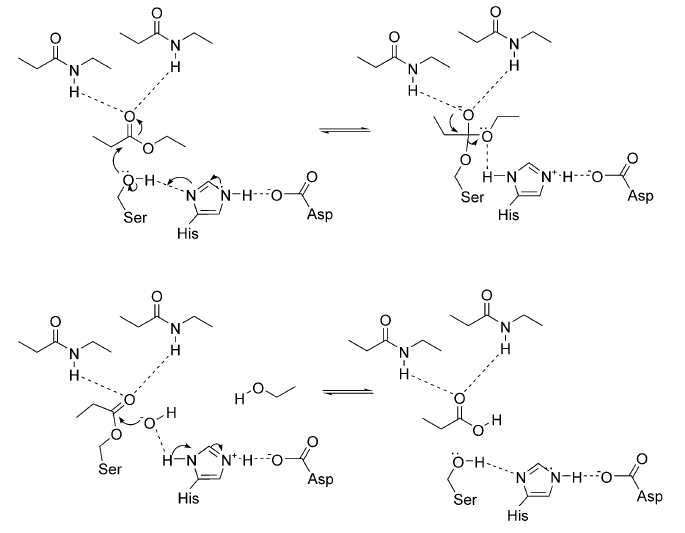
\includegraphics[width=0.7\textwidth]{figures/BSLA_reaction.png}
    \caption{Ester hydrolysis reaction catalyzed by BSLA. Taken from \cite{BSLA_reaction}.}
    \label{fig:BSLAreaction}
\end{figure}  
 
\begin{figure}
    \centering
    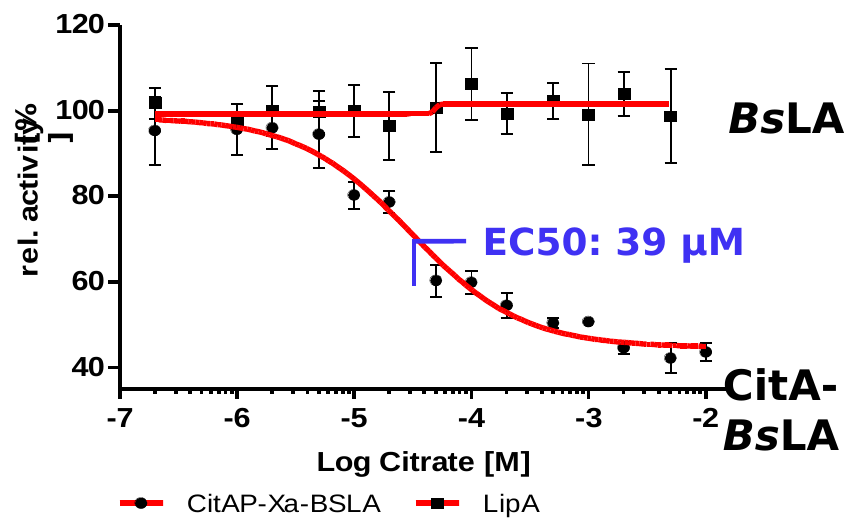
\includegraphics[width=0.5\textwidth]{figures/BSLA_activity/BSLA_activity.png}
    \caption{The activity of the BSLA--CitAP complex is reduced after citrate addition while the uncomplexed lipase is not affected.
    EC50 indicates the concentration of ligand that causes a half-maximal effect (here: change in lipolytic activity)
    Experiments performed by Karl Erich Jaeger et al., data unpublished.}   
    \label{fig:BSLAactivity}
\end{figure} 


\section{Introduction}
\section{Proteins Under Investigation}

\section{Methods}
\subsection{Mean-Shift Clustering}
\label{sec:meanShift} 
\subsection{Dimensionality Reduction}
\label{sec:DimRed} 
\section{Simulation Setups}


\section{Results}

\subsection{Uncomplexed CitAP MD}

To arrive at a quantitative description of the CitAP binding pocket geometry, two distances have been defined (Figure \ref{fig:CitA_pocket}).
Leucine 102 occupies the turning point of the minor loop.
Its backbone nitrogen atom forms a hydrogen bond with the citrate molecule when the pocket is in its closed conformation.
Glutamic acid 74 is located opposite to Leucine 102 in the binding pocket and Tyrosine 56 at the bottom of the active site.
From a visual inspection of the open and closed conformations it is apparent that the distances between the backbone nitrogen of Leucine 102 and the \ce{C_{$\alpha$}} atoms of Glutamic acid 74 and Tyrosine 56 give a good geometrical description, as these are minimal in the closed and maximal in the open conformation.
The crystal structure distances of the LEU102:N to TYR56:C$_{\alpha}$ and LEU102:N to GLU74:C$_{\alpha}$ are 9.3 and 9.9 \r{A}ngstrom respectively.

The results of 100 ns molecular dynamics simulations of CitAP with and without a bound citrate molecule are shown in Figure \ref{fig:CitA_opening_distances}.
The starting structure for both simulations was the citrate bound crystal structure, except for the citrate molecule which has been removed for the citrate free simulations.
While the citrate free pocket opens up within nanoseconds and stays in the open conformation for the entire course of the simulation, the citrate interactions in the bound form keep the minor loop tightly closed, covering citrate in the binding pocket.
For the first half of the simulation, the LEU102:N to GLU74:C$_{\alpha}$ distance gets even smaller than the crystal structure reference distance.
This is due to intense hydrogen bonding with the citrate ligand and the absence of crystal packing artifacts in solution.
After approximately 50 ns, the two distances cross in the right panel of Figure \ref{fig:CitA_opening_distances}, meaning that the LEU102:N to TYR56:C$_{\alpha}$ distance now gets slightly longer than before and the LEU102:N to GLU74:C$_{\alpha}$ slightly shorter.
This is however not of influence on the binding interactions of citrate.
Figure \ref{fig:CitAP_dist_hist} shows the same distance data for the LEU102 - GLU74 distance in a histogram to verify that the distributions are continuous and not build up of multiple stable conformations.

\begin{figure}
    \centering
    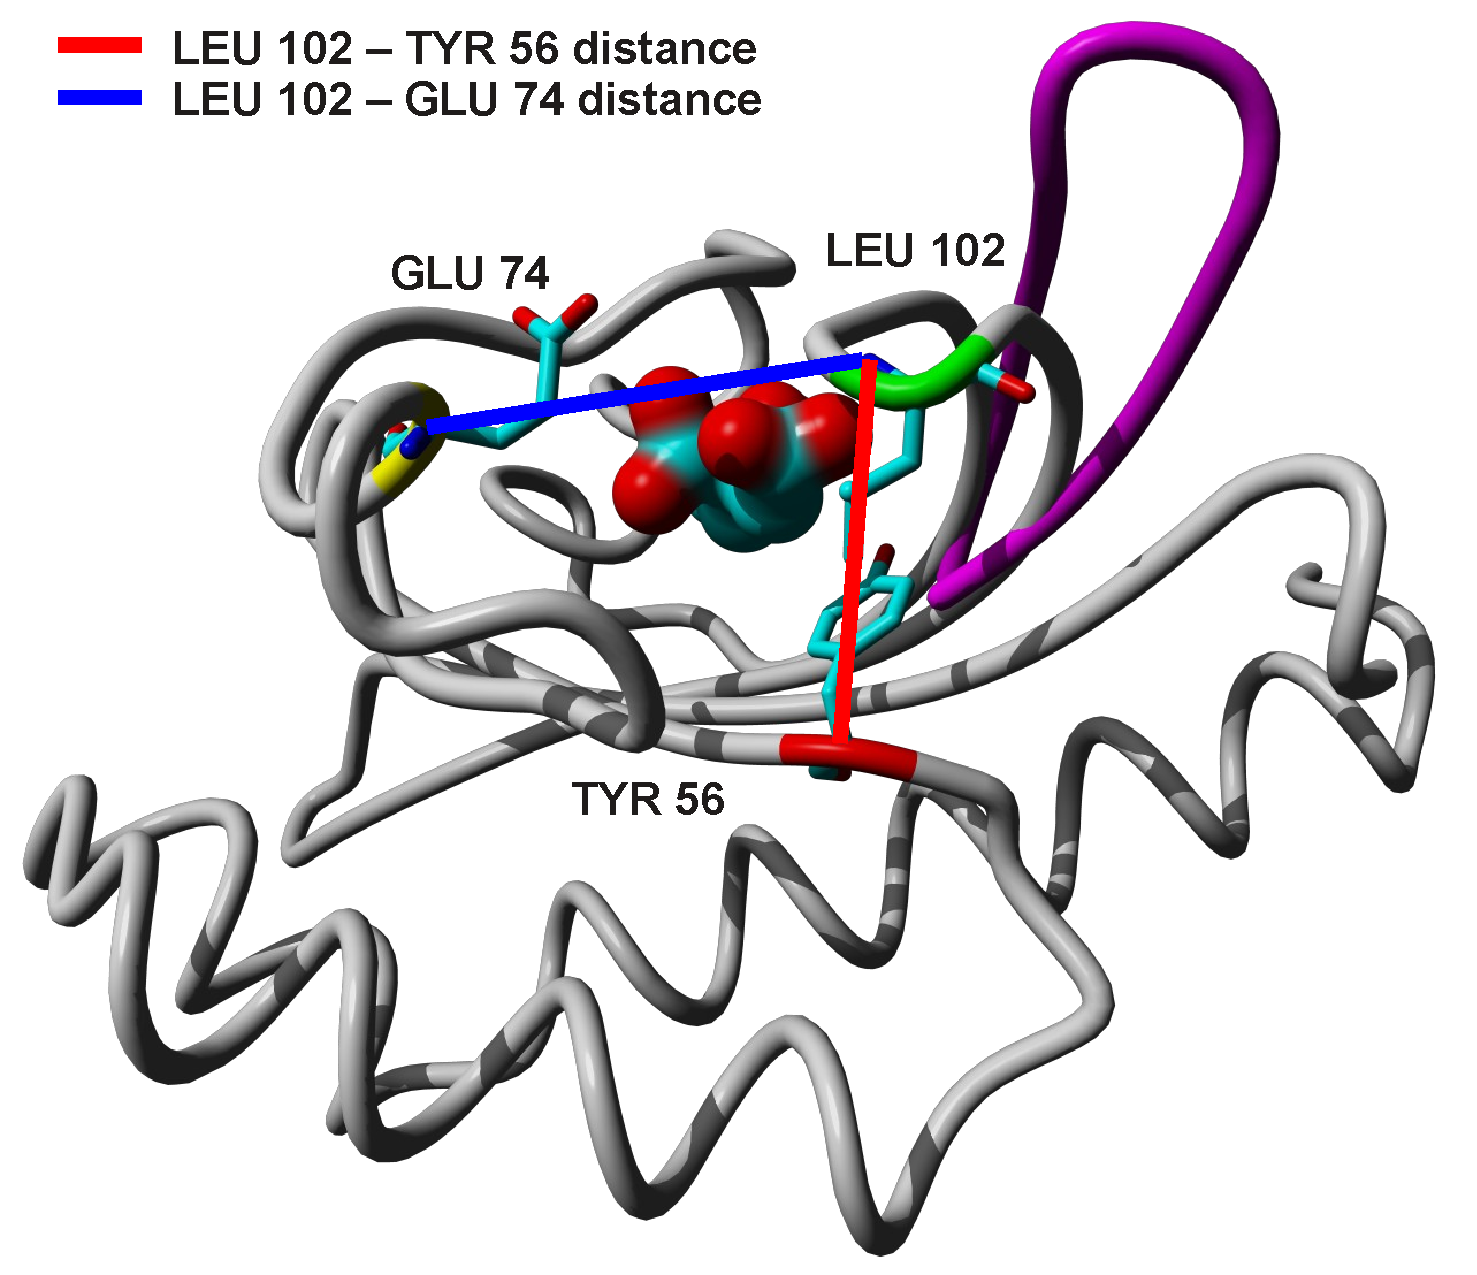
\includegraphics[width=0.7\textwidth]{figures/CitA_pocket2.pdf}
    \caption{To measure the geometry of the CitAP binding pocket, two distances were introduced: The distance between the backbone nitrogen of Leucine 102 and the \ce{C_{$\alpha$}} atoms of Glutamic acid 74 (blue) and Tyrosine 56 (red).
    The purple loop shows the minor loop in the fully extended open conformation.}
    \label{fig:CitA_pocket}
\end{figure}        

\begin{figure}
    \begin{minipage}[]{0.45\linewidth}
        \centering
        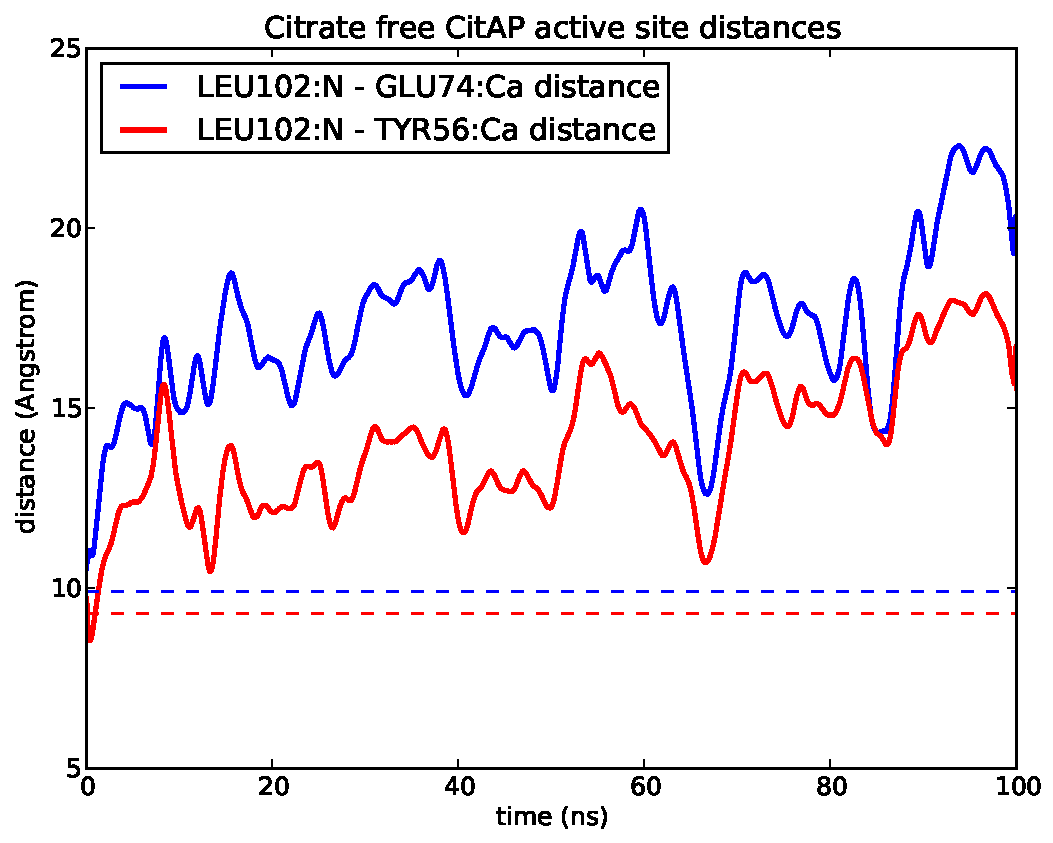
\includegraphics[width=1.0\textwidth]{figures/CitAP_opening/CitAP_dist_free.pdf}
    \end{minipage}
\hspace{0.5cm}
    \begin{minipage}[]{0.45\linewidth}
        \centering
        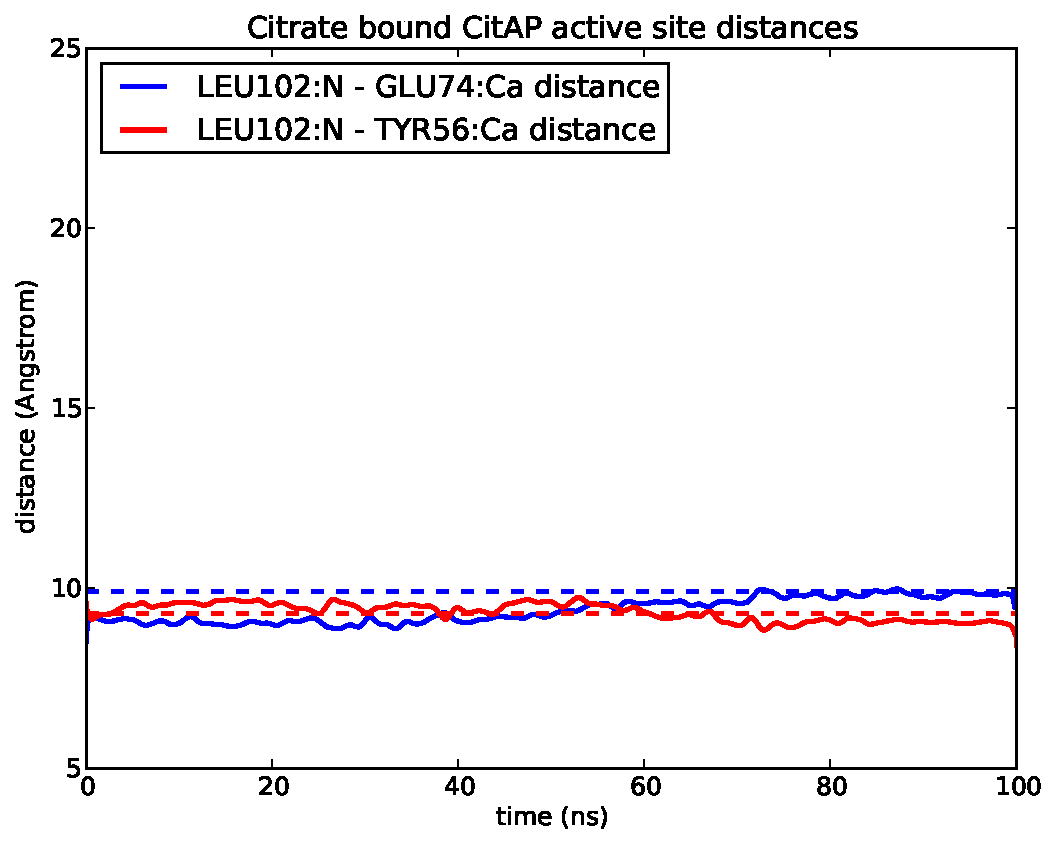
\includegraphics[width=1.0\textwidth]{figures/CitAP_opening/CitAP_dist_bound.pdf}
    \end{minipage}
    \caption{The plot shows the distances defined in Figure \ref{fig:CitA_pocket} (same color coding) during 100 ns MD trajectories. The respective distances in the crystal structures are drawn with a dashed line. The left panel corresponds to the citrate free, the right panel to the citrate bound case.}
\label{fig:CitA_opening_distances}
\end{figure}        

\begin{figure}
    \centering
    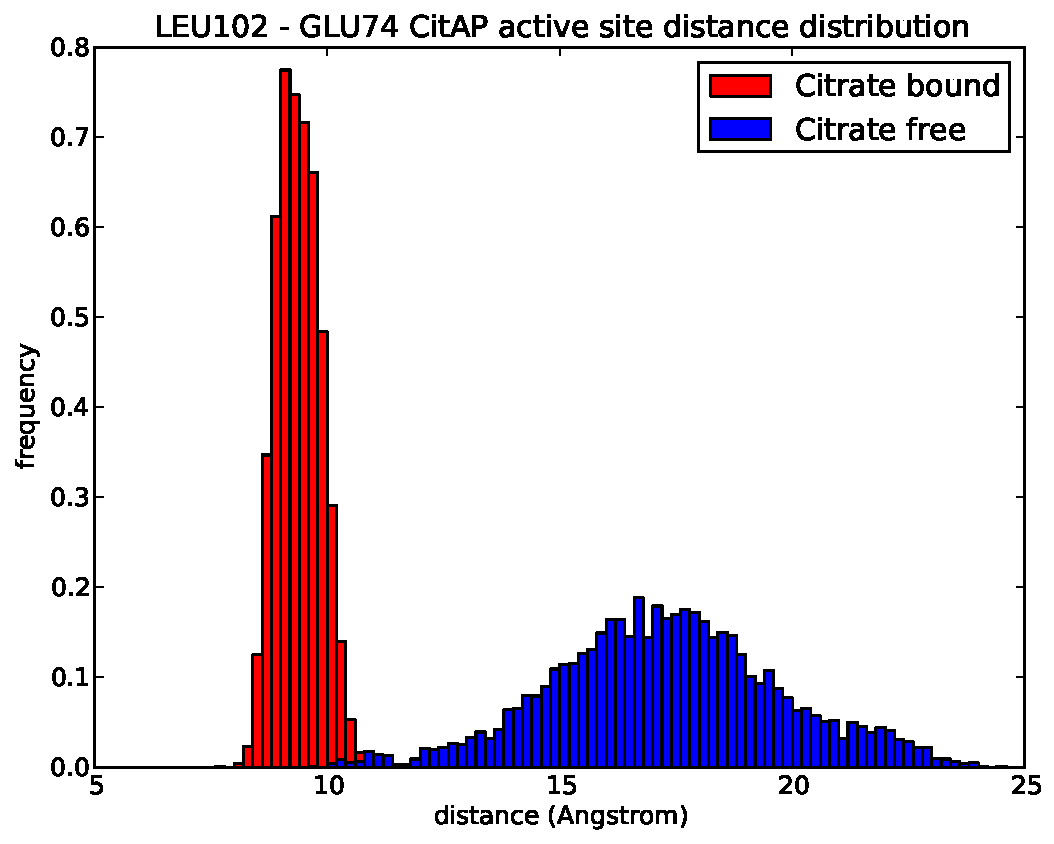
\includegraphics[width=0.7\textwidth]{figures/CitAP_opening/CitAP_dist_hist_both.pdf}
    \caption{Distributions of the LEU102:N - GLU74:G$_{\alpha}$ distance for the citrate free and bound simulations.
    Both distributions have been normalized to integrate to 1.}
    \label{fig:CitAP_dist_hist}
\end{figure}         

%\begin{figure}
%    \centering
%    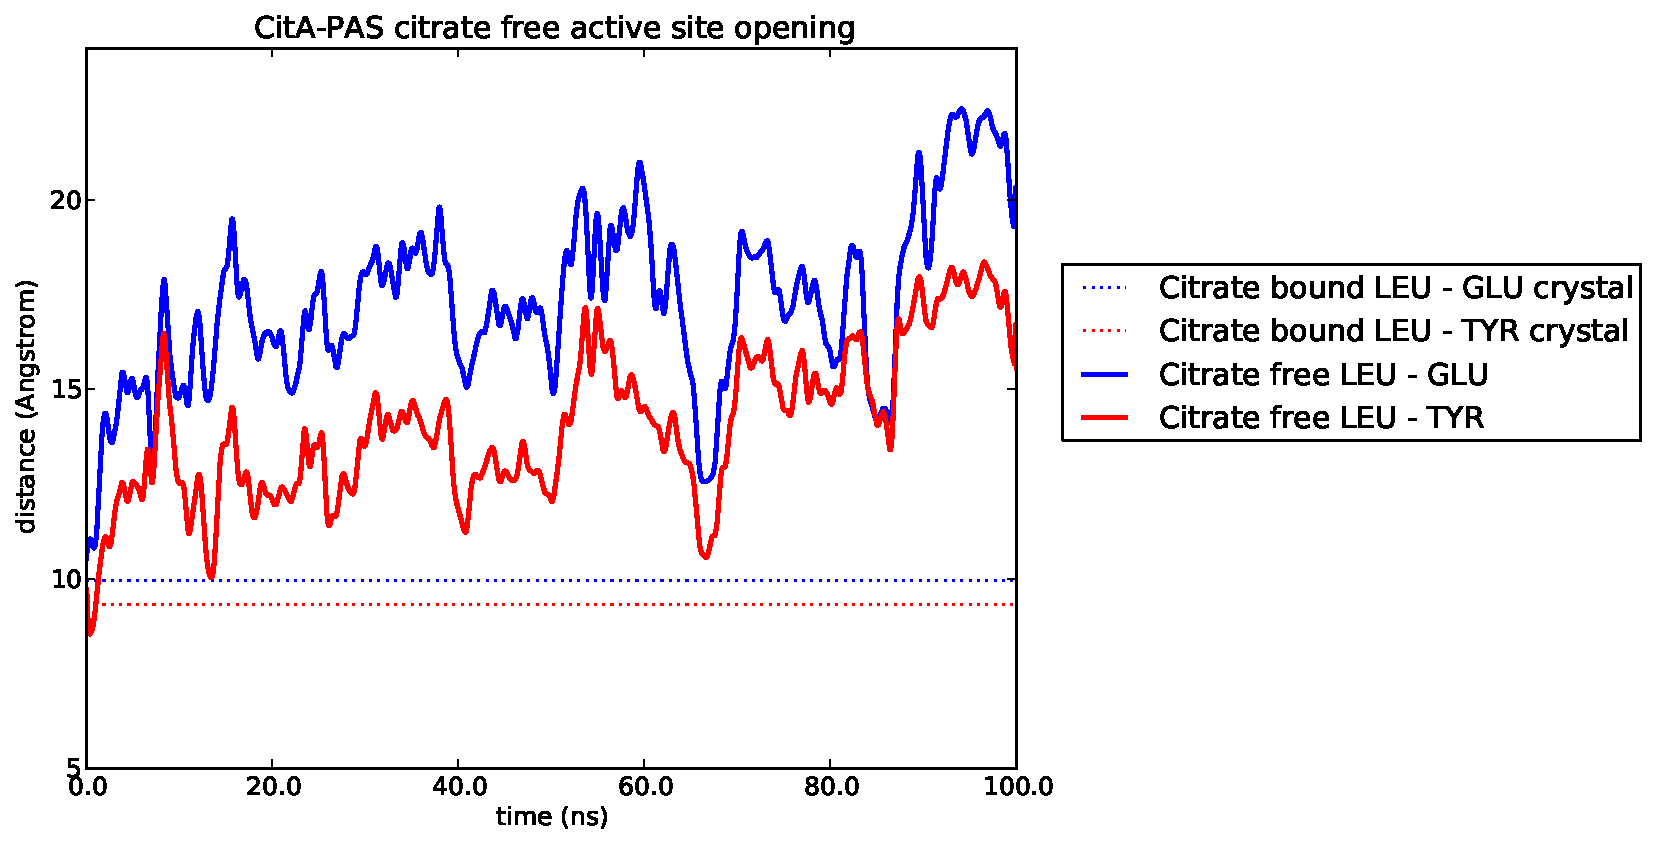
\includegraphics[width=1.0\textwidth]{figures/CitAP_opening/CitA_opening_citrate_free.pdf}
%    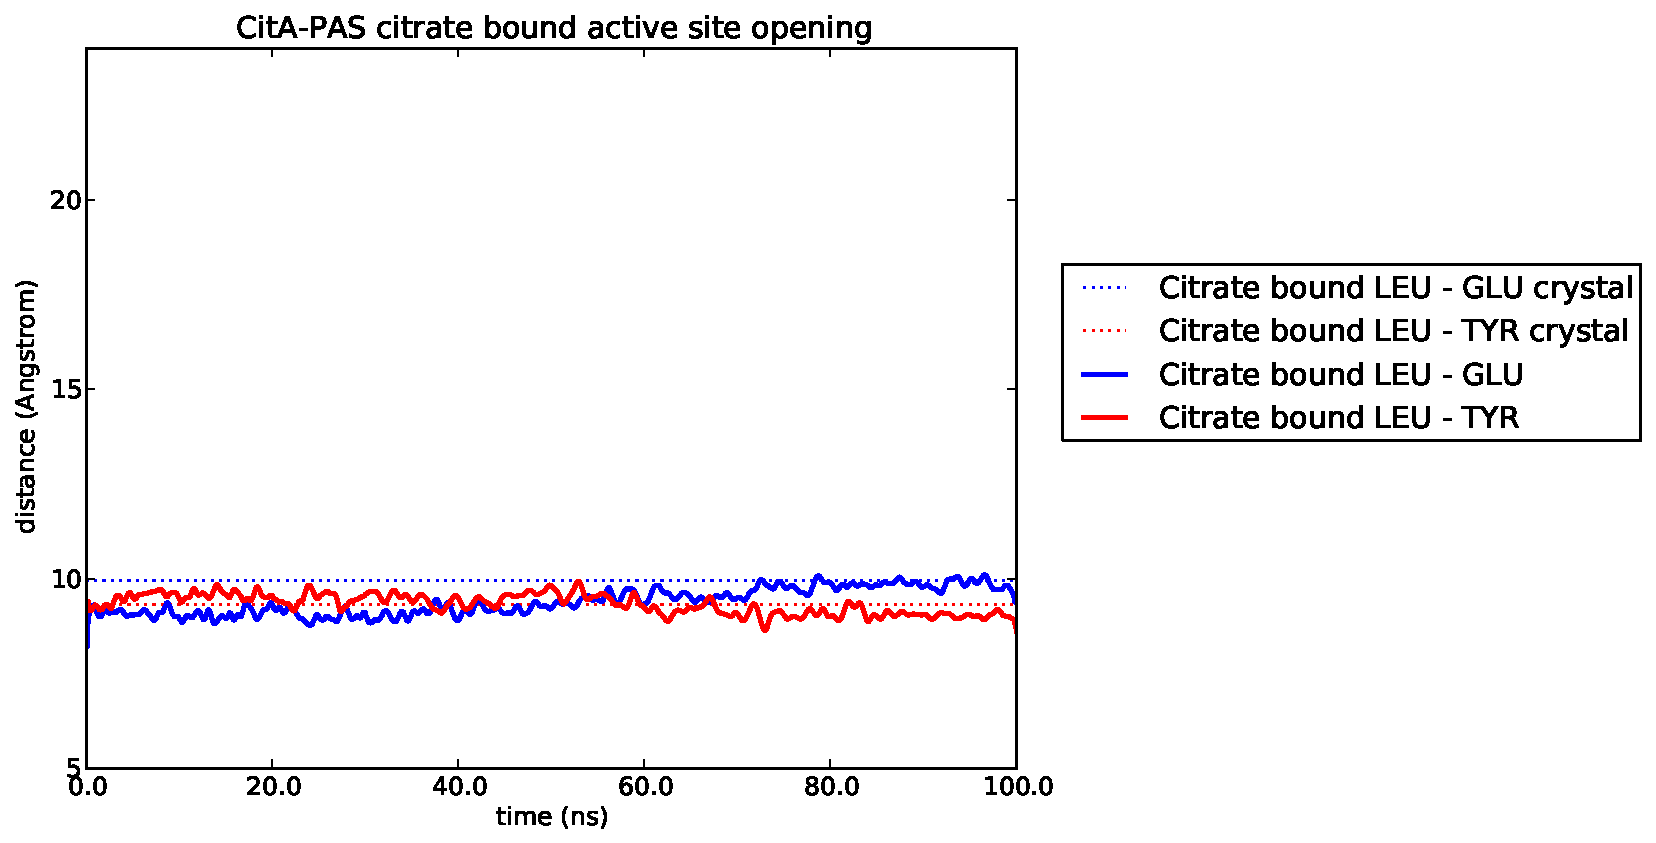
\includegraphics[width=1.0\textwidth]{figures/CitAP_opening/CitA_opening_citrate_bound.pdf}
%    \caption{The plot shows the distances defined in Figure \ref{fig:CitA_pocket} (same color coding) during 100 ns MD trajectories. The respective distances in the crystal structures are drawn with a dashed line. The top panel corresponds to the citrate free, the bottom panel to the citrate bound case.}
%    \label{fig:CitA_opening_distances}
%\end{figure}       



\subsection{Uncomplexed BSLA MD}

BSLA is very stable in solution during a 100 ns MD simulation.
Figure \ref{fig:BSLA_solo} a) shows the root mean square fluctuation (RMSF) of the C$_{\alpha}$ atoms.
The core structure has an RMSF around 0.5 \r{A}ngstrom and the average RMSF over all C$_{\alpha}$ atoms is 0.55 \r{A}ngstrom.
All residues with an RMSD larger than 1.0 \r{A}ngstrom are colored red in Figure \ref{fig:BSLA_flexibility}.
These residues are located at the C and N termini, as well as at solvent exposed turns.
Turns are generally more likely to be flexible than other secondary structure elements like helices and $\beta$-sheets, therefore this result shows the inherent stability of the uncomplexed BSLA structure.
Figure \ref{fig:BSLA_solo} b) shows the minimum distance between the side chains of ASP133 and HIS156 at the active site of BSLA.
Hydrogen bonding between these residues stabilizes the intermediate tetrahedral structure during ester hydrolysis (Figure \ref{fig:BSLAreaction}).
This distance might therefore be indicative for disruption of the active site geometry of BSLA resulting in a drop in activity.
The minimum distance of the uncomplexed BSLA is very stable and close to the crystal structure distance during the MD trajectory with a standard deviation of only 0.07 \r{A}ngstrom.
The histogram of Figure \ref{fig:BSLA_solo} b) gives an impression of the distribution of the minimum ASP133 - HIS156 distance.
The variance in the active site distance distribution serves as a baseline for the complexed structure and its disruption is assumed to be indicative for lipase activity degradation.



\begin{figure}
    \begin{minipage}[]{0.45\linewidth}
        \centering
        a)
        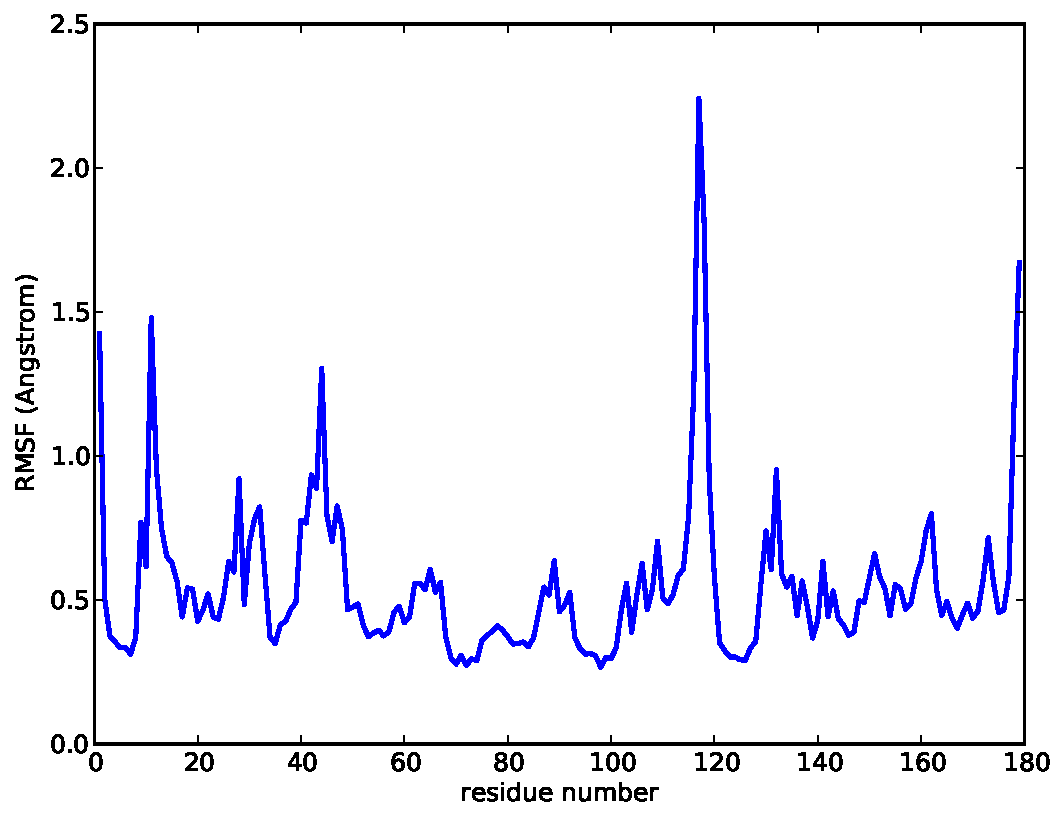
\includegraphics[width=\textwidth]{figures/BSLA_solo/BSLA_solo_rmsf.pdf}  
    \end{minipage}
\hspace{0.5cm}
    \begin{minipage}[]{0.45\linewidth}
        \centering
        b)
        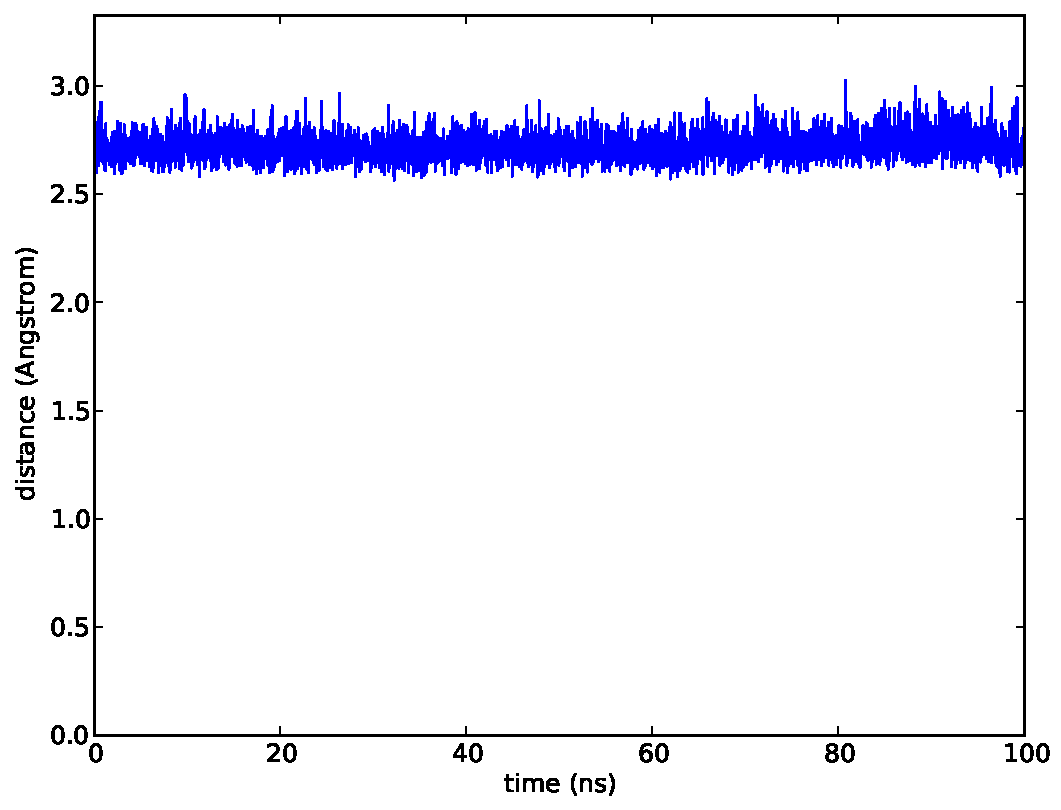
\includegraphics[width=\textwidth]{figures/BSLA_solo/BSLA_solo_dist_ASP133_HIS156.pdf} 
        c)
        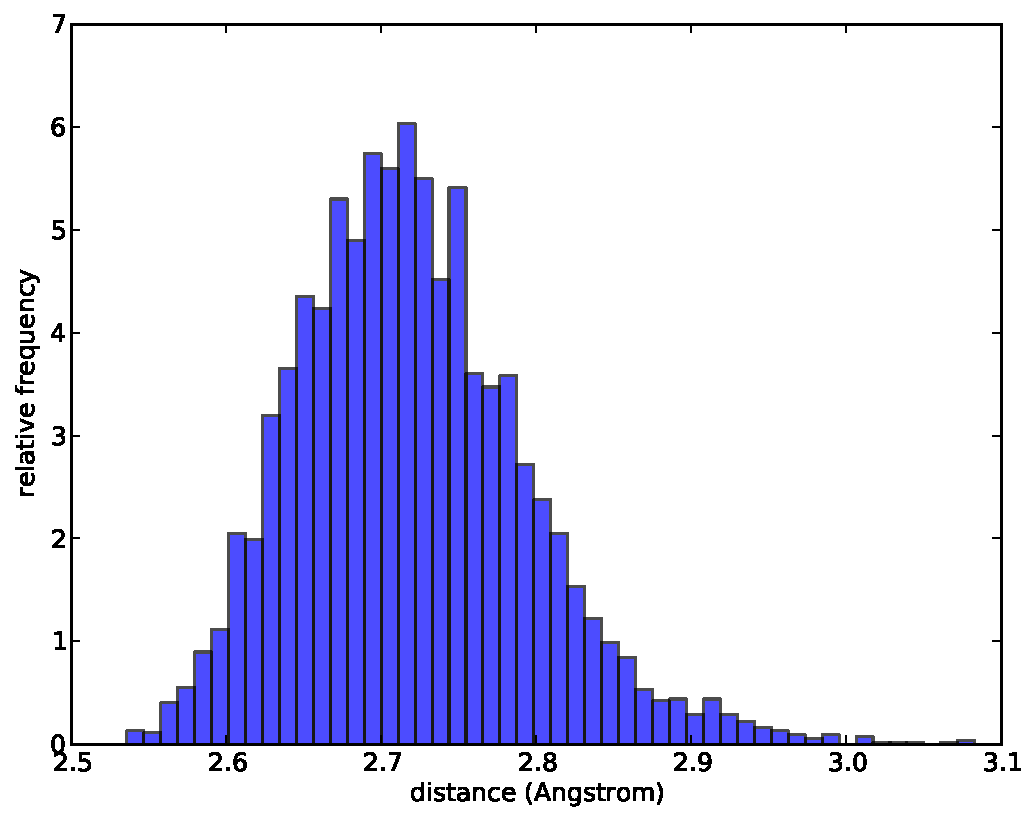
\includegraphics[width=\textwidth]{figures/BSLA_solo/BSLA_distribution_ASP133_HIS156.pdf}  
    \end{minipage}
    \caption{
    \textbf{a)} Root mean square fluctuation (RMSF) of C$_\alpha$ atoms around the average structure of the 100 ns MD trajectory.
    \textbf{b)} Shortest distance between side chain atoms of BSLA active site residues ASP133 and HIS156 during a 100 ns MD trajectory. 
    \textbf{c)} Distribution of the distance from a).}
\label{fig:BSLA_solo}
\end{figure} 


\begin{figure}
    \centering
    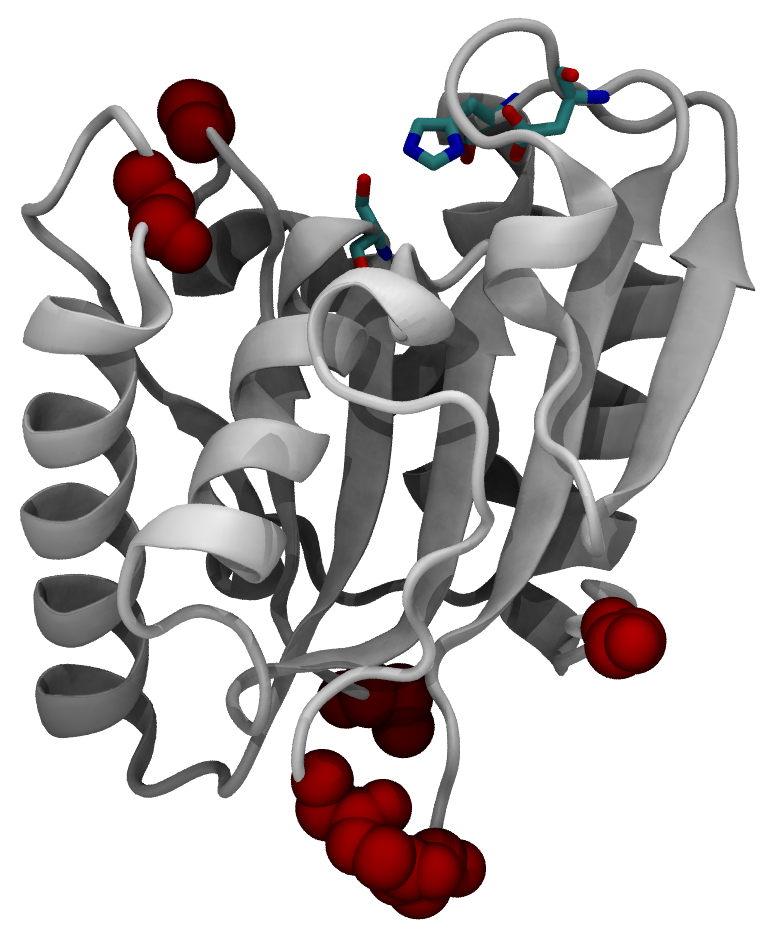
\includegraphics[width=0.5\textwidth]{figures/BSLA_flexibility.png}
    \caption{The structure of BSLA is shown in cartoon representation. The flexible parts with an RMSF larger than 1.0 \r{A} are shown in red Van-der-Waals representation. The active site residues are colored.}
    \label{fig:BSLA_flexibility}
\end{figure}       
 




\subsection{Complex Basin Hopping}

The 12 Basin Hopping runs each resulted in 10 possible structures for the fusion protein.
To arrive at a small set on which to perform molecular dynamics simulations, these 120 structures were clustered with the mean shift clustering algorithm, as described in section \ref{sec:meanShift}.
Before clustering, the spatial coordinates have been transformed into a reduced coordinate space of two sets of spherical coordinates as described in section \ref{sec:DimRed}.
These spherical coordinates, together with the energy of each structure as a separate coordinate, where the input space in which clustering was performed.
Figure \ref{fig:GMIN_CitA_phi} gives an impression of the reduction of the dataset due to clustering.
The grey points represent the original dataset and the colored points the reduced dataset, which consists of only 18 points.
When adapting the mean shift window parameter to further reduce the number of clusters, too many features of the dataset got lost due to assignment to the same cluster.


\begin{figure}
    \centering
    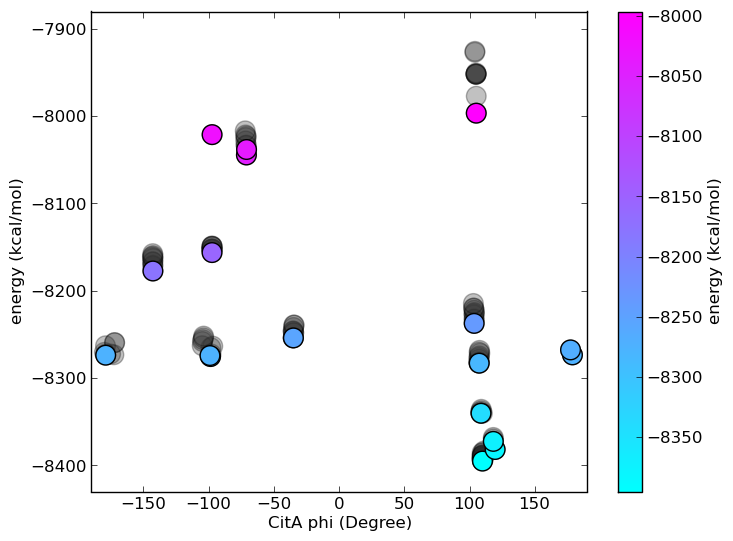
\includegraphics[width=0.7\textwidth]{figures/CitA_phi.png}
    \caption{GMIN output structures before (grey) and after clustering (colored).
        The CitA phi angle denotes the spherical $\phi_{Complex}$ angle from the reduced coordinate set.
        y-axis and color coding both represent the energy of each structure.}
    \label{fig:GMIN_CitA_phi}
\end{figure}        

It should be noted that the grey points in Figure \ref{fig:GMIN_CitA_phi} coincide almost part with the colored points.
This is due to the fact that GMIN runs with different parameters often arrived at very similar energy minima.
Figure \ref{fig:GMIN_results} shows a three dimensional plot of the BSLA centers of mass around superpositions of CitAP domains in order to give an impression of the distribution of the structures after clustering.
Each BSLA structure in addition has a unique orientation with respect to the position of CitAP.
Four structures have been selected for further investigation.
Table \ref{tab:GMIN_structures} lists all GMIN output structures with their corresponding energies and Basin Hopping parameters.
The structures shaded in grey are the four selected output structures.
Structure 3 and 5 have been skipped as they were found to be too similar to already selected structures by visual inspection.
The mean shift clustering algorithm assigned those two structures to separate clusters because the energy was used as a separate coordinate during clustering and their energy differs from structures that would be in the same cluster base solely on the reduced spherical coordinates.
The four output structures used for the fusion protein MD simulations are shown in Figure \ref{fig:GMIN_output}.
In structure 1 the active site of CitAP faces the BSLA domain, effectively restricting its minor loop movement.
Structures 2 and 3 also make contact with their CitAP active site and the BSLA domain, although less severe than in structure 1.
In structure 4 the CitAP active site faces away from the BSLA domain and has therefore the largest conformational freedom.
The BSLA active site is in all four structures freely accessible.

\begin{figure}
    \centering
    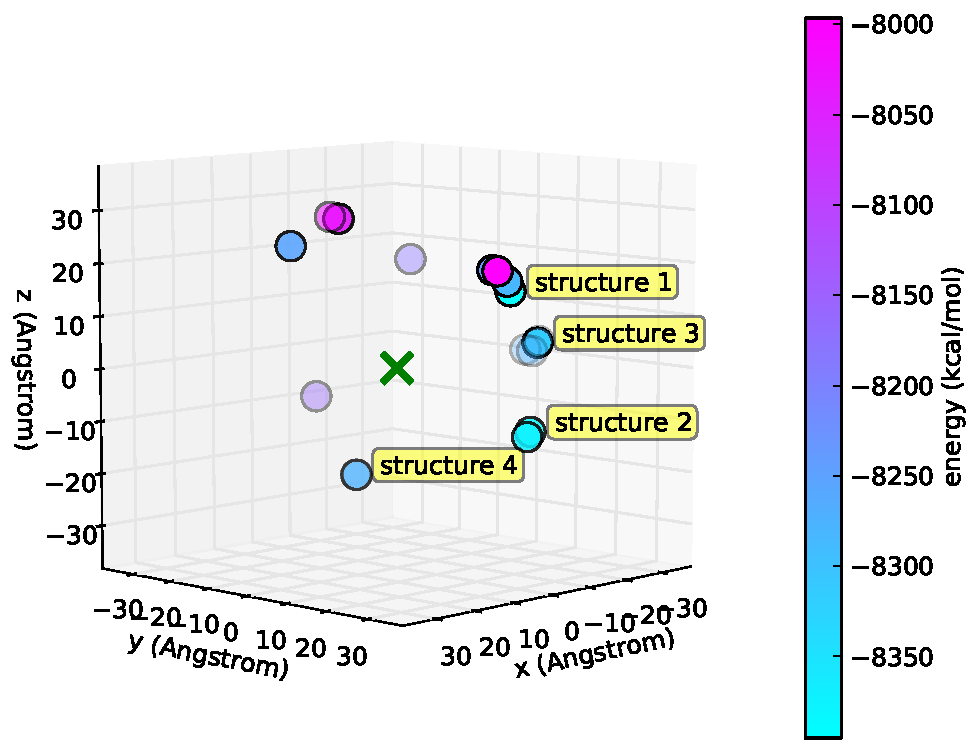
\includegraphics[width=1.0\textwidth]{figures/GMIN/CitA_phi_theta_3D.pdf}
    \caption{Cluster centers of the GMIN output structures. The green cross indicates the center of mass position of the superimposed CitAP domains. The points correspond to the centers of mass of the BSLA domains of each GMIN output structure. Color codes the energy of the structures as indicated by the color bar and the transparency is used as a depth cue. The four structures used in subsequent experiments are labeled.}
    \label{fig:GMIN_results}
\end{figure}       


 

\begin{table}
\centering
\begin{tabular}{c c c c c}
    \hline \hline
    Energy     & BH steps & Max. angular step & Convergence Crit. & GMIN run \\ 
    (kcal/mol) &          & size (degree)     & (kcal/mol)        & rank     \\
    \hline
    \rowcolor{lightgray}
    -8395.14   & 10000    &  90               & 0.02              & 1        \\ 
    \rowcolor{lightgray}
    -8381.87   &   500    &  60               & 0.02              & 1        \\
    -8372.59   &   500    &  60               & 0.02              & 2        \\
    \rowcolor{lightgray}
    -8340.34   &   500    &  60               & 0.02              & 6        \\
    -8282.96   &  1000    &  90               & 0.02              & 1        \\
    \rowcolor{lightgray}
    -8275.37   &   500    & 120               & 0.02              & 1        \\
    -8274.22   &   500    & 120               & 0.02              & 2        \\
    -8273.80   &   500    &  30               & 0.02              & 1        \\
    -8273.46   &   500    &  30               & 0.02              & 2        \\
    -8267.76   &   500    &  30               & 0.02              & 7        \\
    -8254.04   &  1000    &  90               & 0.05              & 1        \\
    -8237.37   &   500    &  90               & 0.02              & 1        \\
    -8177.33   &   500    &  90               & 0.02              & 1        \\
    -8156.23   &  1000    &  90               & 0.1               & 1        \\
    -8044.41   &   100    &  90               & 0.02              & 1        \\
    -8038.14   &   100    &  90               & 0.02              & 2        \\
    -8021.09   &   100    &  90               & 0.02              & 9        \\
    -7996.48   &  1000    &  90               & 0.5               & 1        \\
    \hline \hline
\end{tabular}
\caption{Representative structures for the clusters of GMIN output structures, ranked according to the lowest energy.
The number of Basin Hopping (BH) steps, the maximum angular step size and the convergence criterium for the energy minimization are given, as well as the rank of each structure in the GMIN run in which they have been obtained.
    The four structures used in subsequent experiments are shaded in grey and referenced in the text according to their enumeration as structures 1 to 4.}
\label{tab:GMIN_structures}
\end{table} 




% GMIN output structures
\begin{figure}
    \begin{minipage}[]{0.45\linewidth}
        \centering
        1)
        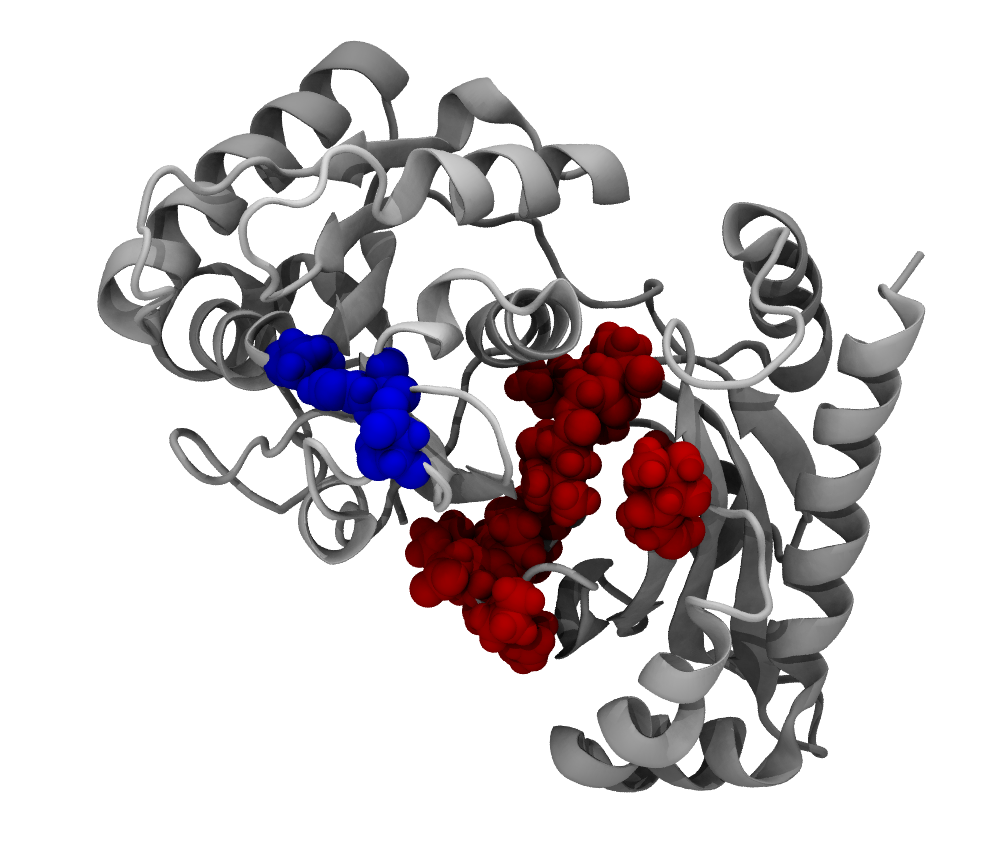
\includegraphics[width=\textwidth]{figures/Complex_structures/structure1.png}  
        3)
        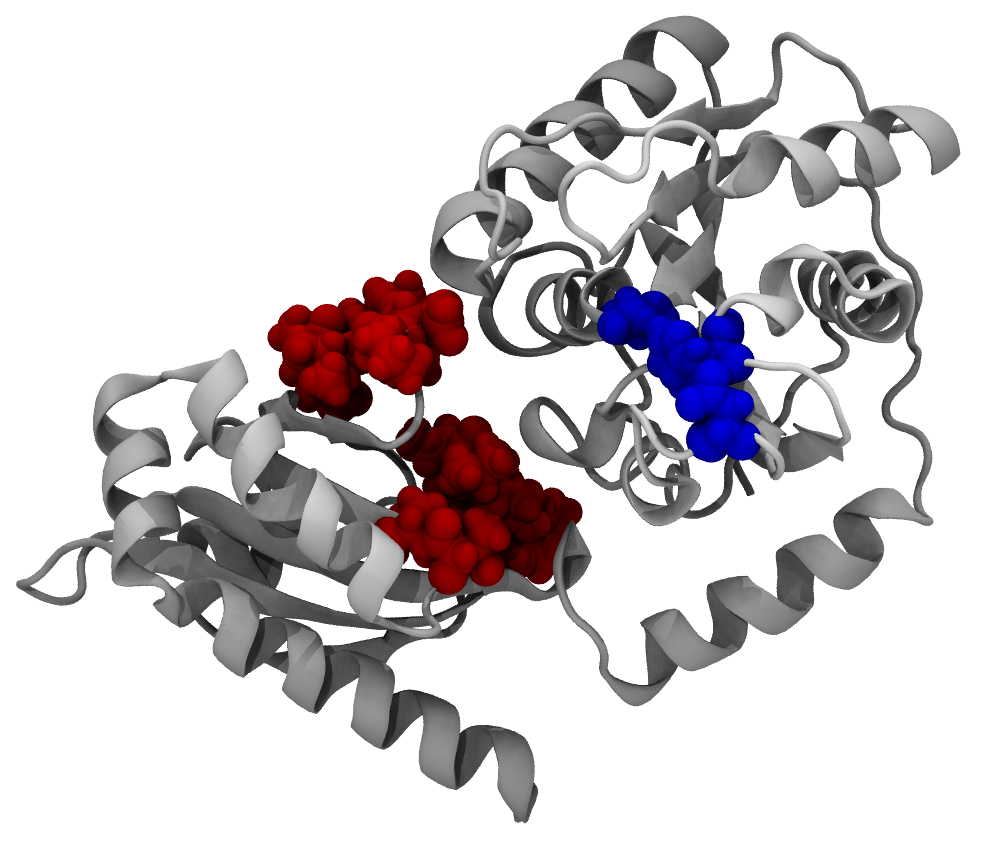
\includegraphics[width=\textwidth]{figures/Complex_structures/structure3.png}  
    \end{minipage}
\hspace{0.5cm}
    \begin{minipage}[]{0.45\linewidth}
        \centering
        2)
        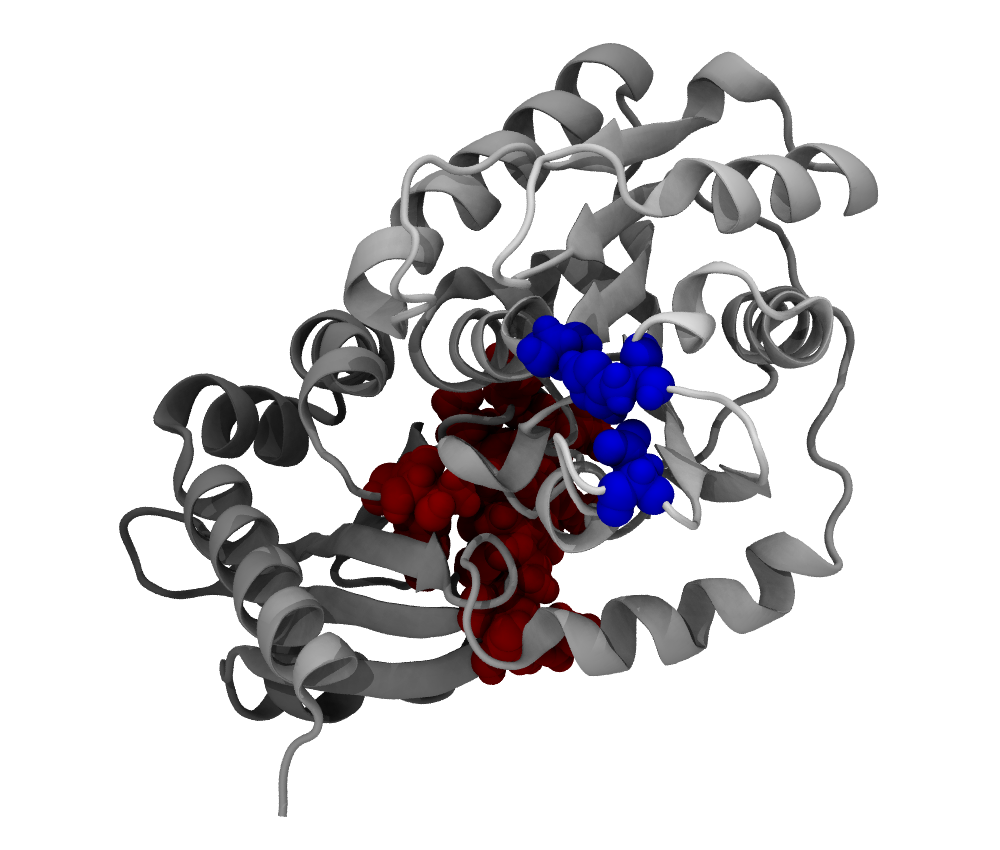
\includegraphics[width=\textwidth]{figures/Complex_structures/structure2.png}  
        4)
        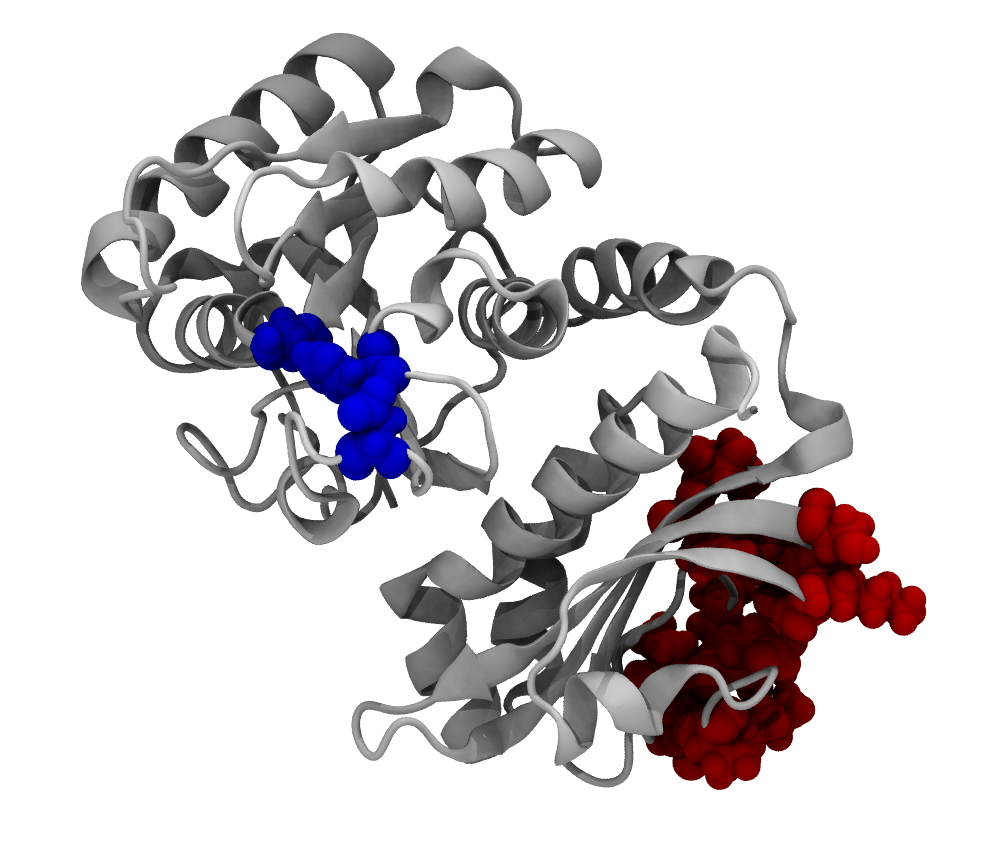
\includegraphics[width=\textwidth]{figures/Complex_structures/structure4.png}  
    \end{minipage}
    \caption{The fours selected output structures.
        The BSLA active site residues are shown in blue and the CitAP active site is shown in red.
        The BSLA domains have been superimposed to indicate the relative CitAP conformations.
    The structures are numbered from 1 to 4.}
\label{fig:GMIN_output}
\end{figure}       




\subsection{CitAP--BSLA fusion protein MD}

The first important property of interest that is accessible by molecular dynamics simulation is the general stability of the fusion protein.
This has been addressed on more than one scale.
The secondary structure of the complexes has been estimated with the DSSP program \cite{DSSPalgorithm, DSSPwebsite}.
Figure \ref{fig:DSSP_bound} shows the secondary structure evolution during the course of 100 ns MD runs for the citrate bound simulations, Figure \ref{fig:DSSP_free} displays the same for the citrate free cases.
The secondary structure of the fusion protein is remarkably stable during all simulations and hardly any structure gets lost, apart from some minor fluctuations.
Only during the citrate free simulation of structure 2, the fifth $\alpha$-helix vanishes and forms a turn.
This helix is very small, located at the solvent interface and surrounded by unstructured coils and therefore one of the least stable secondary structure elements in the fusion protein.
The linker helix remains stable in all four structures, whether citrate bound or citrate free.


% bound DSSP
\begin{figure}
    \centering
    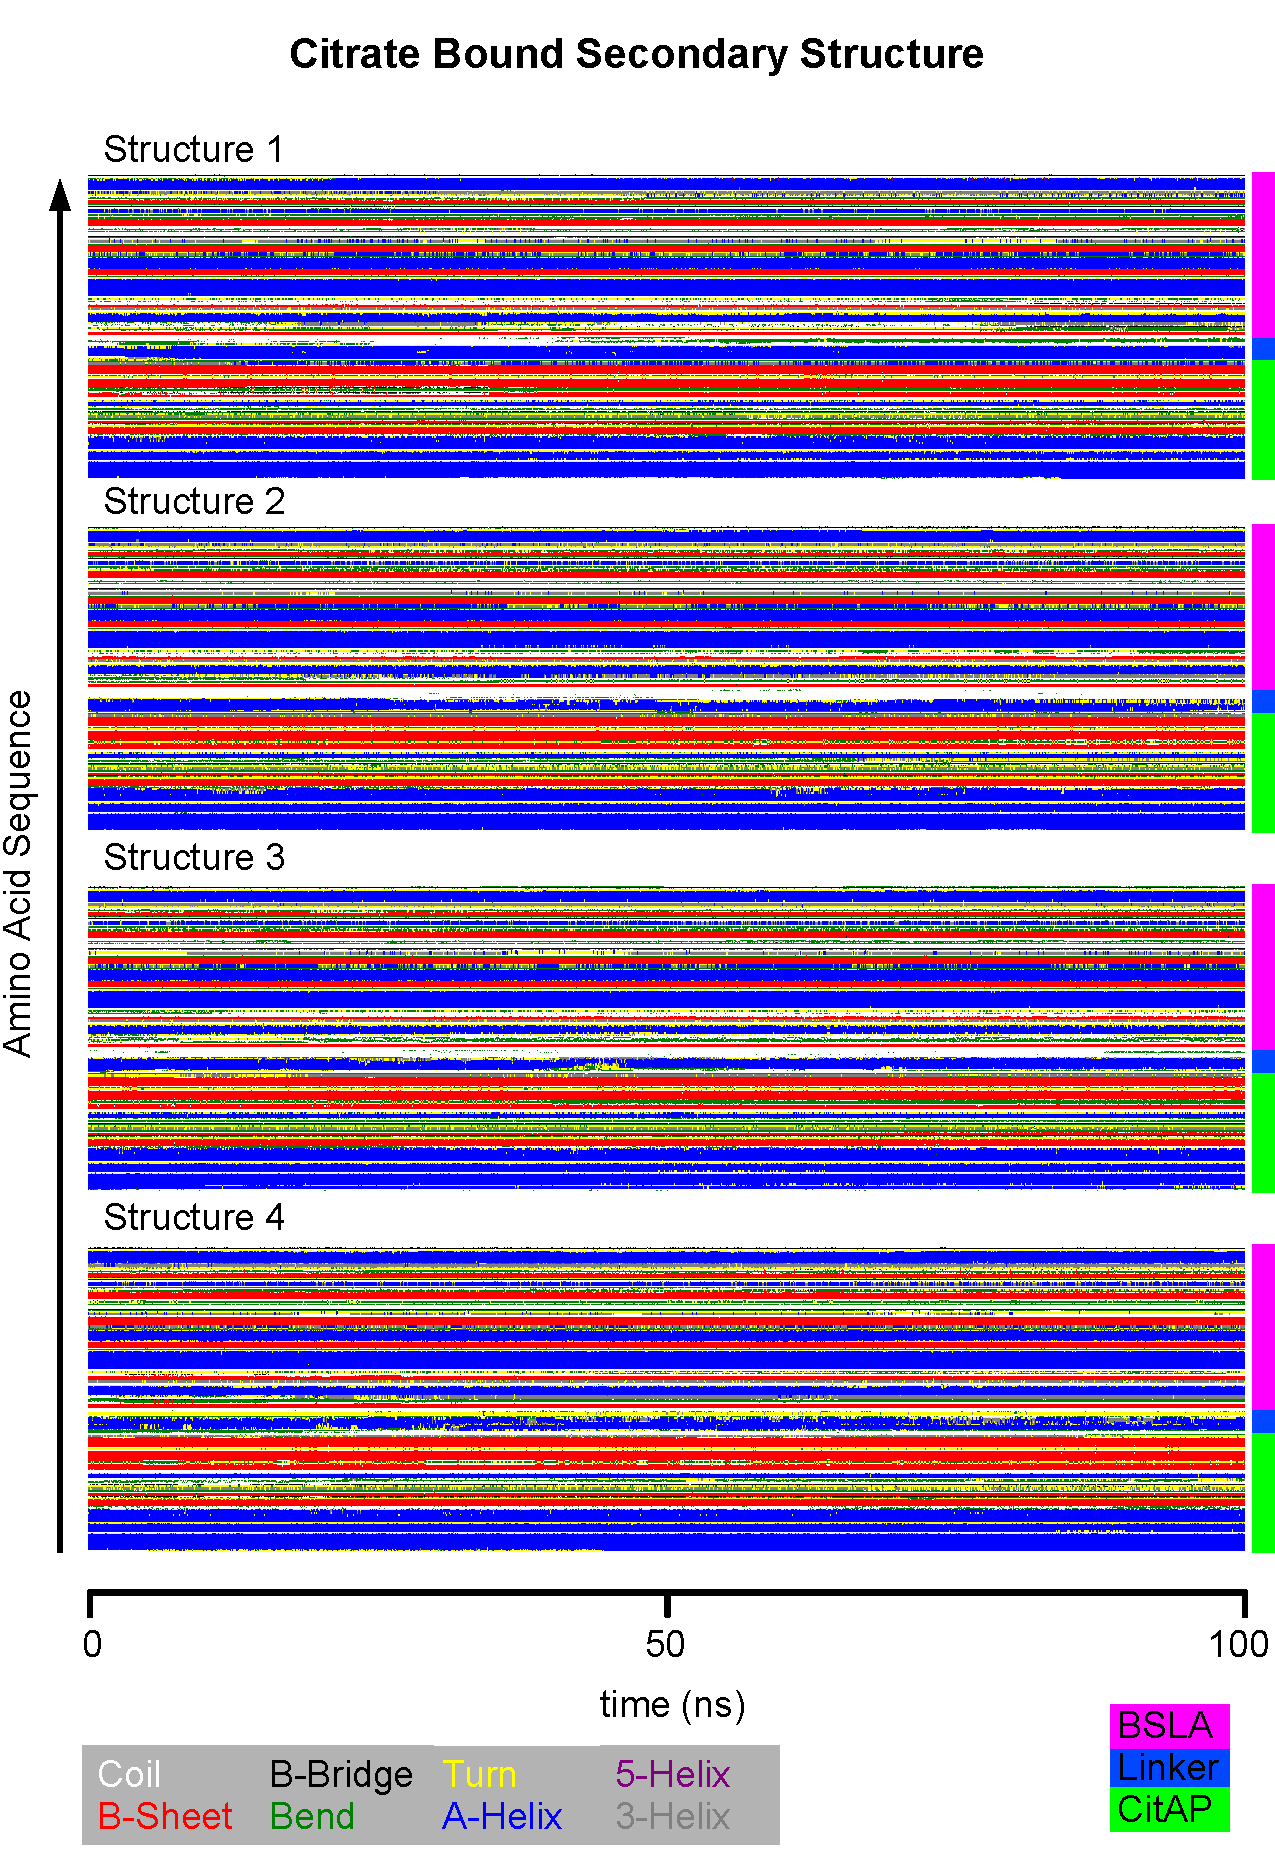
\includegraphics[width=0.9\textwidth]{figures/DSSP/dssp_bound.pdf}
    \caption{Secondary structure of the citrate bound complexes.}
    \label{fig:DSSP_bound}
\end{figure}          



% free DSSP
\begin{figure}
    \centering
    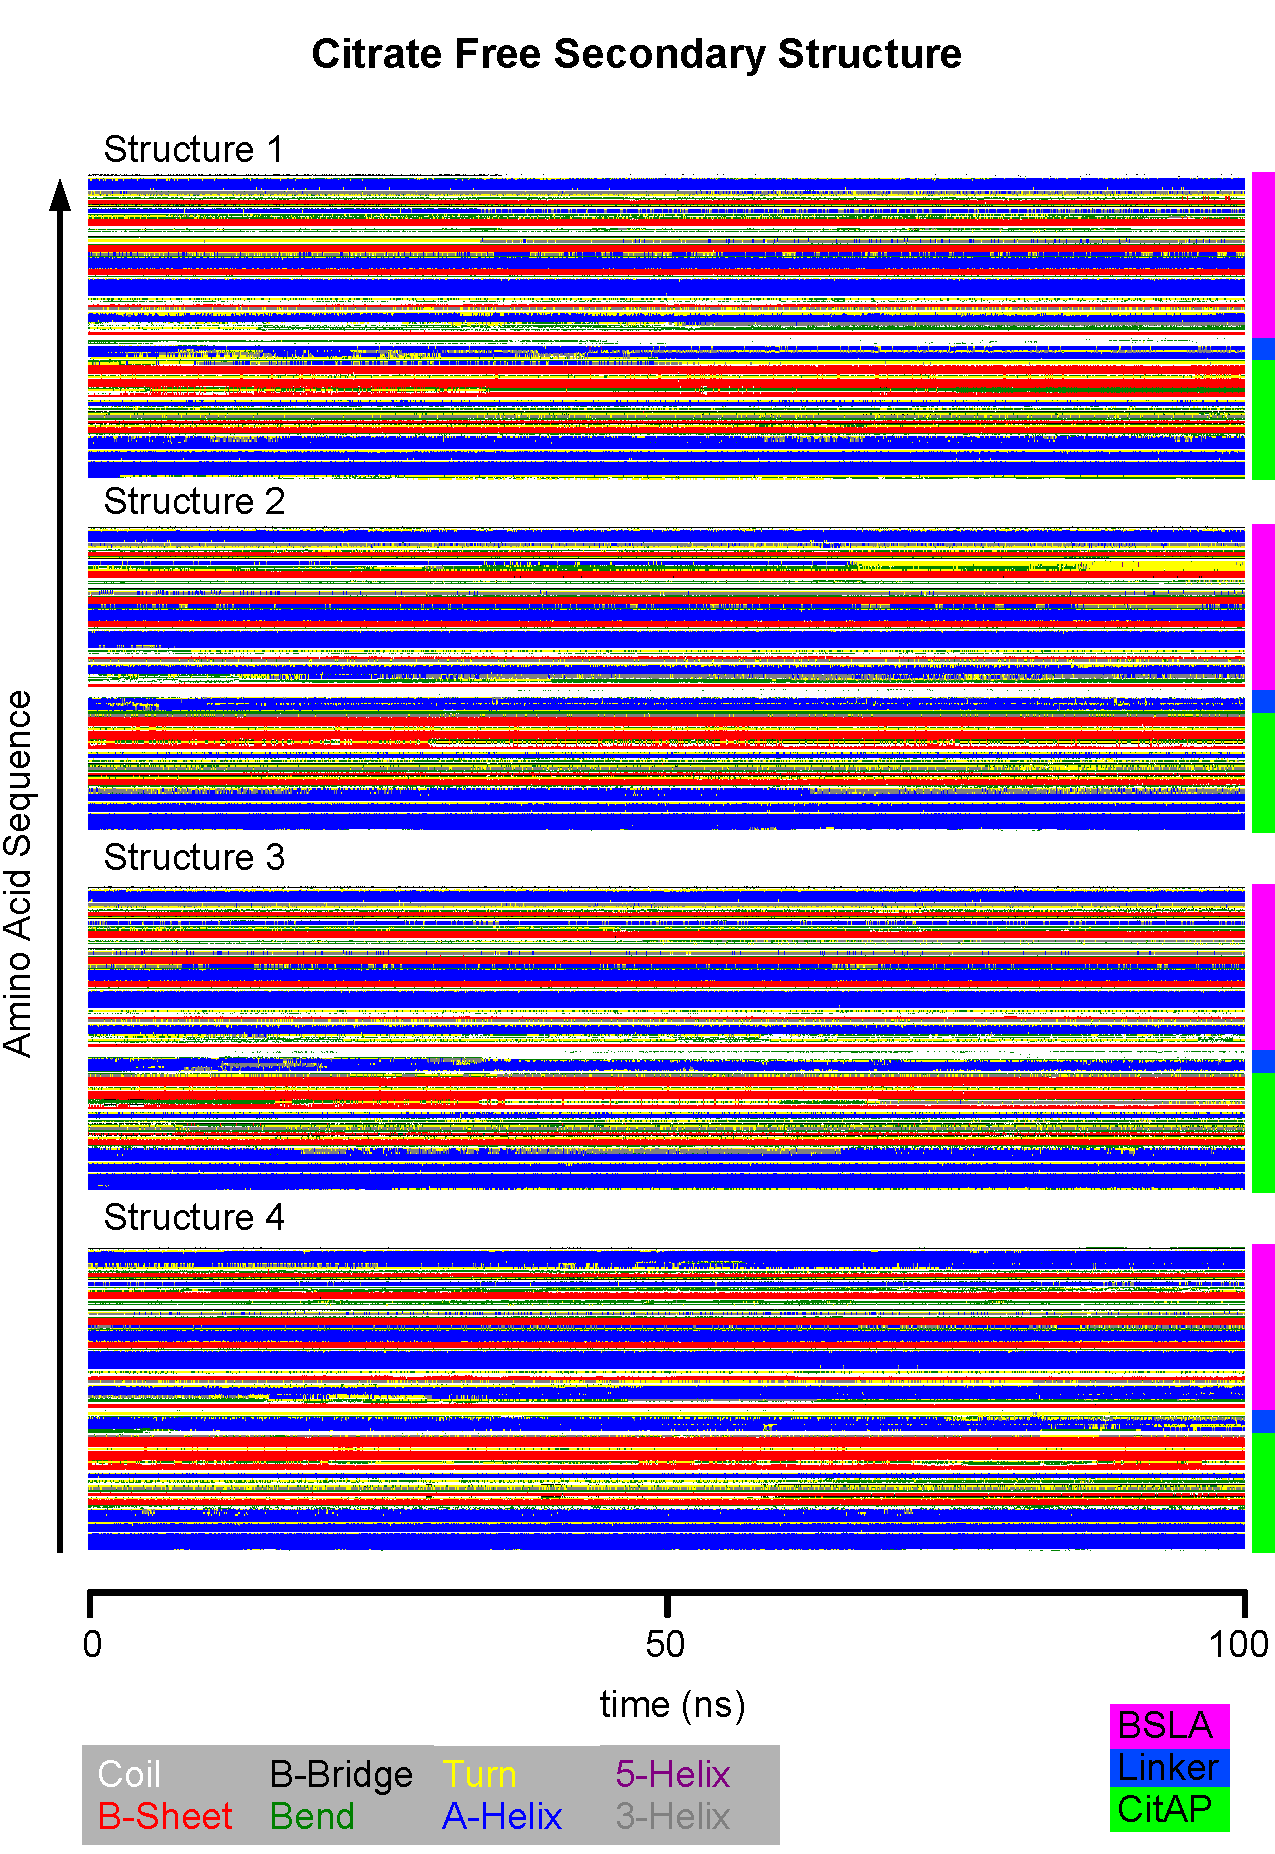
\includegraphics[width=0.9\textwidth]{figures/DSSP/dssp_free.pdf}
    \caption{Secondary structure of the citrate free complexes.}
    \label{fig:DSSP_free}
\end{figure}



To obtain a more detailed view on the way in which the CitAP and BSLA domains interact, the hydrophobic and hydrophilic interactions have been investigated.
Figure \ref{fig:favourable_contacts} shows the favourable contacts between the two domains as a fraction of inter-domain contacts.
Favourable is here defined as contacts between two residues that are either both hydrophobic or both hydrophilic and a contact between a hydrophobic and a hydrophilic group is therefore viewed as unfavourable.
This is a simplified view that most importantly does not take into account contacts between side chains with the same charge, which are particularly unfavourable, but as these are very rare, they contribute very little to the final result.
In all citrate free structures the fraction of favourable contacts increases during the course of the simulation slightly.
For the citrate bound simulations, this effect is less pronounced and for structure 1 and 3 the number of favourable contacts even decreases.



% favourable contacts
\begin{figure}
    \begin{minipage}[]{0.45\linewidth}
        \centering
        a)
        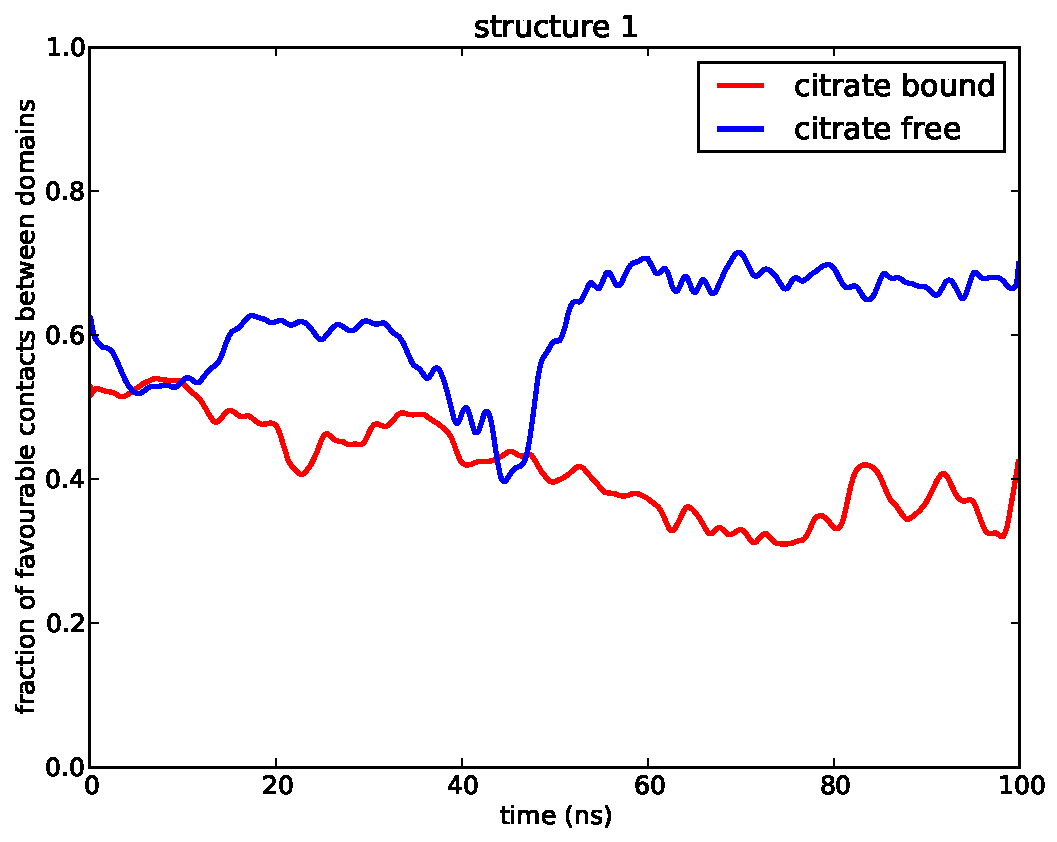
\includegraphics[width=\textwidth]{figures/Complex_hydrophobic_core/favourable_cont_structure1.pdf}  
        c)
        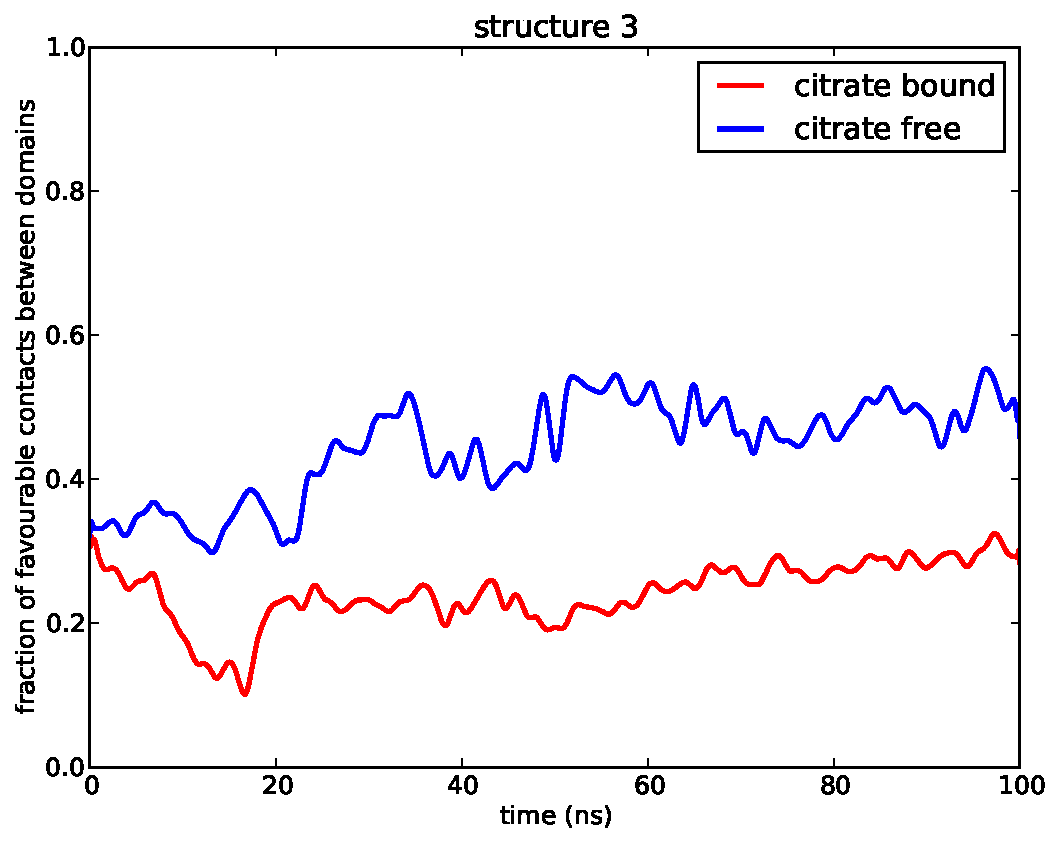
\includegraphics[width=\textwidth]{figures/Complex_hydrophobic_core/favourable_cont_structure3.pdf}  
    \end{minipage}
\hspace{0.5cm}
    \begin{minipage}[]{0.45\linewidth}
        \centering
        b)
        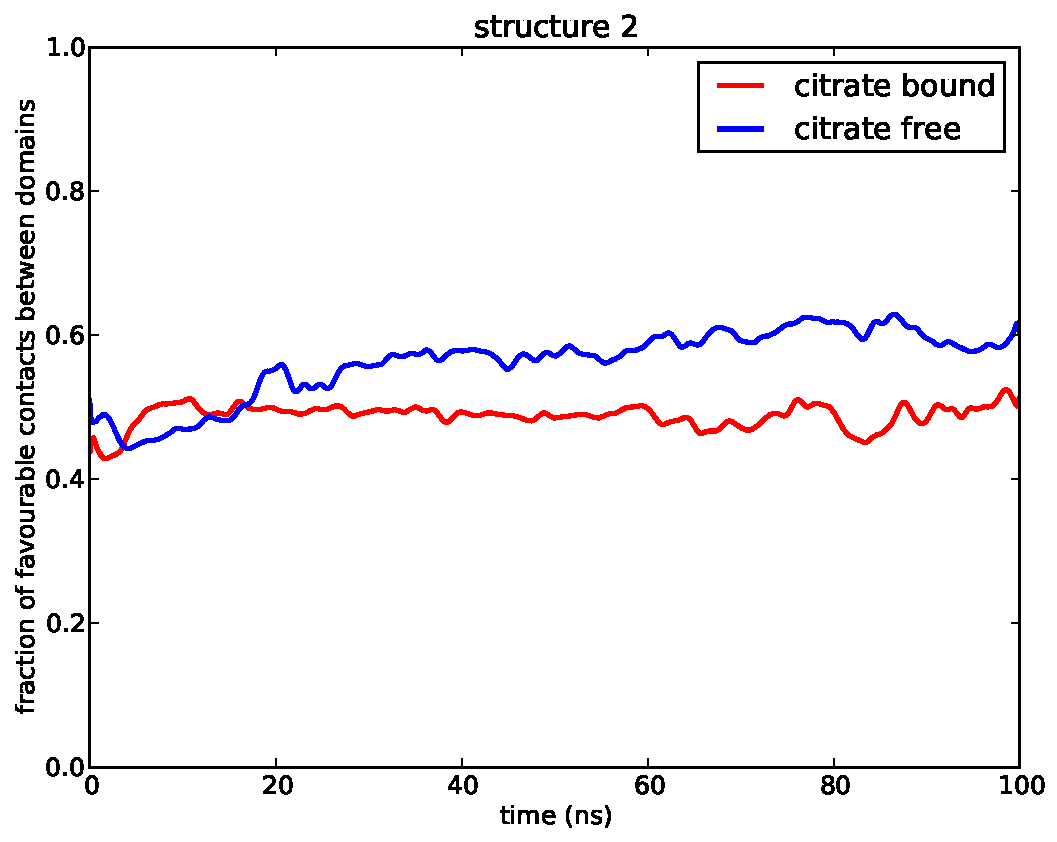
\includegraphics[width=\textwidth]{figures/Complex_hydrophobic_core/favourable_cont_structure2.pdf}  
        d)
        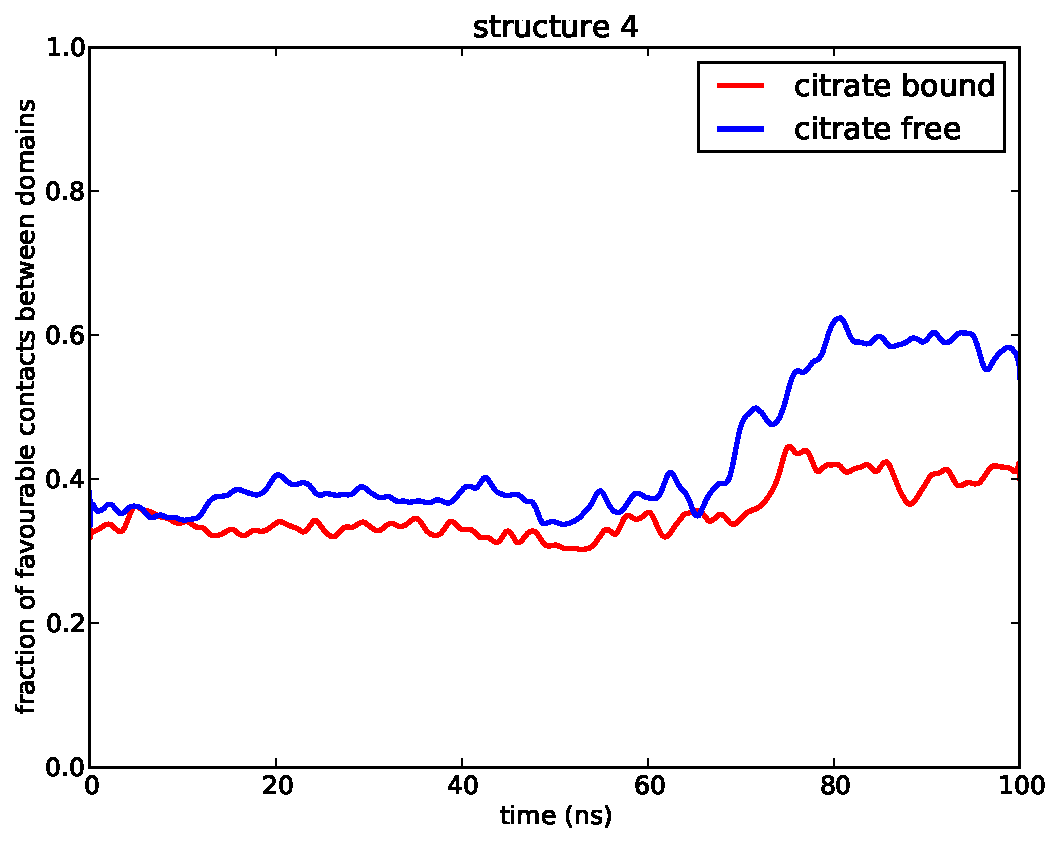
\includegraphics[width=\textwidth]{figures/Complex_hydrophobic_core/favourable_cont_structure4.pdf}  
    \end{minipage}
    \caption{Fraction of favourable contacts (i.e. hydrophobic to hydrophobic and hydrophilic to hydrophilic) of the total number of contacts between the CitAP and BSLA domains.
        The data has been smoothed by a Gaussian window function to remove high frequent fluctuations for better visualizability.}
\label{fig:favourable_contacts}
\end{figure}   



The general theme of the structure of globular proteins is a mostly hydrophobic core surrounded by a hydrophilic shell.
This is also true for the two proteins under study, with the exception of the inside of the CitAP binding pocket, which is hydrophilic to accommodate the charged citrate.
Figure \ref{fig:hydrophobic_contacts} shows the fraction of hydrophobic contacts of all inter-domain interactions in the fusion protein during the MD simulations.
In all four structures the number of hydrophobic contacts in the interface region is relatively low, with the tendency to increase slightly in the course of the simulation.
As for the favourable contacts, this effect is more pronounced for the citrate free structures.
It is interesting to note that by design all structures have a conformation with two separated domains corresponding to the original proteins, each with its own hydrophobic core (Figure \ref{fig:hydrophobic_core}).
These cores stay mostly isolated during the simulation, even though there are hydrophobic patches at which the two domains could attach to each other.




% hydrophobic contacts
\begin{figure}
    \begin{minipage}[]{0.45\linewidth}
        \centering
        a)
        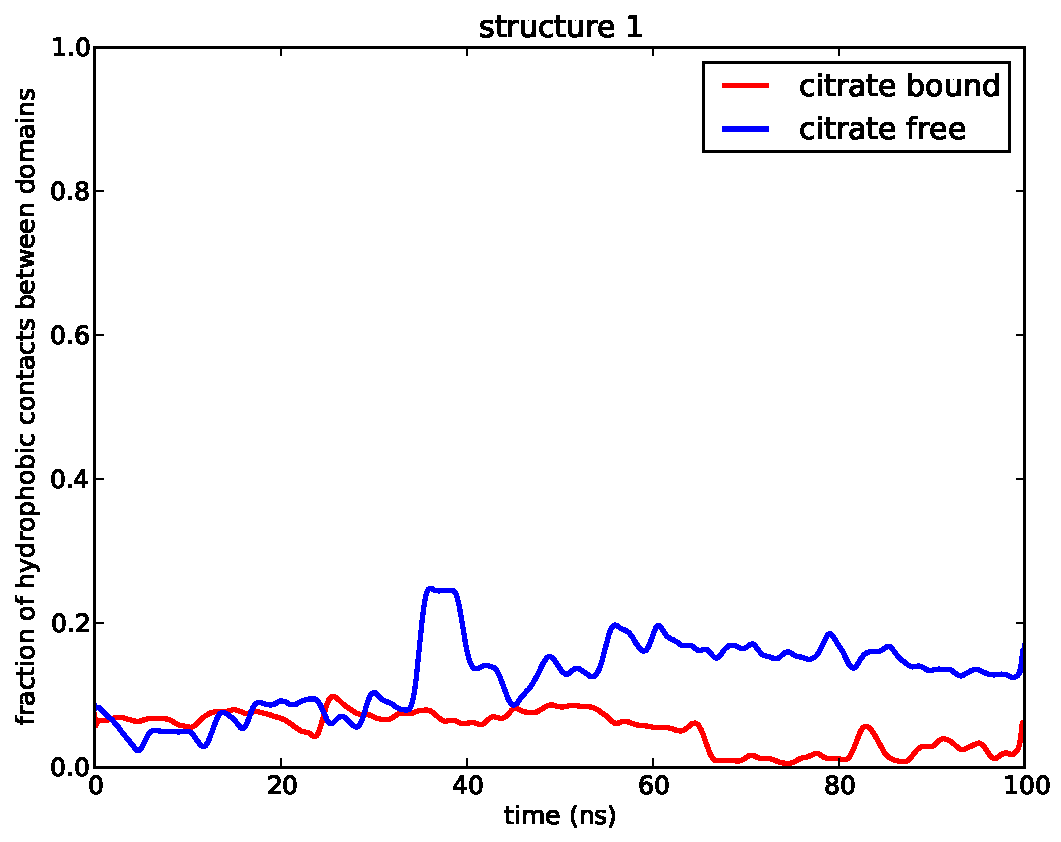
\includegraphics[width=\textwidth]{figures/Complex_hydrophobic_core/hydrophobic_cont_structure1.pdf}  
        c)
        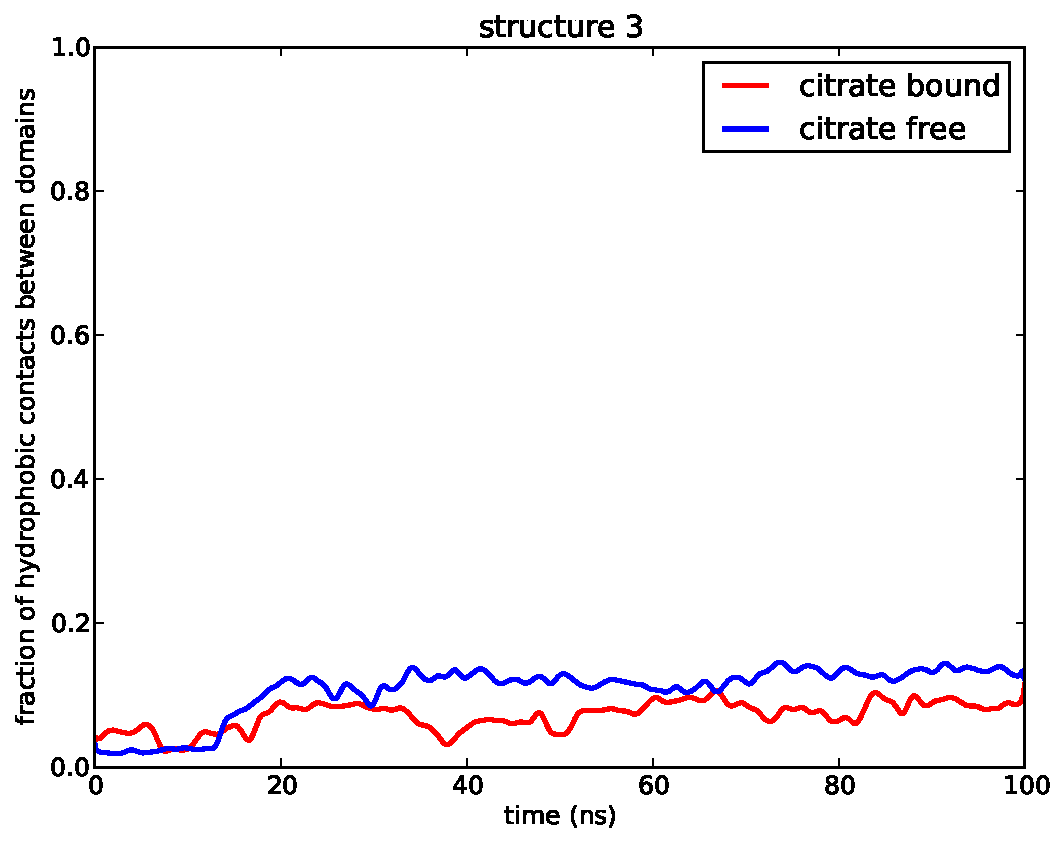
\includegraphics[width=\textwidth]{figures/Complex_hydrophobic_core/hydrophobic_cont_structure3.pdf}  
    \end{minipage}
\hspace{0.5cm}
    \begin{minipage}[]{0.45\linewidth}
        \centering
        b)
        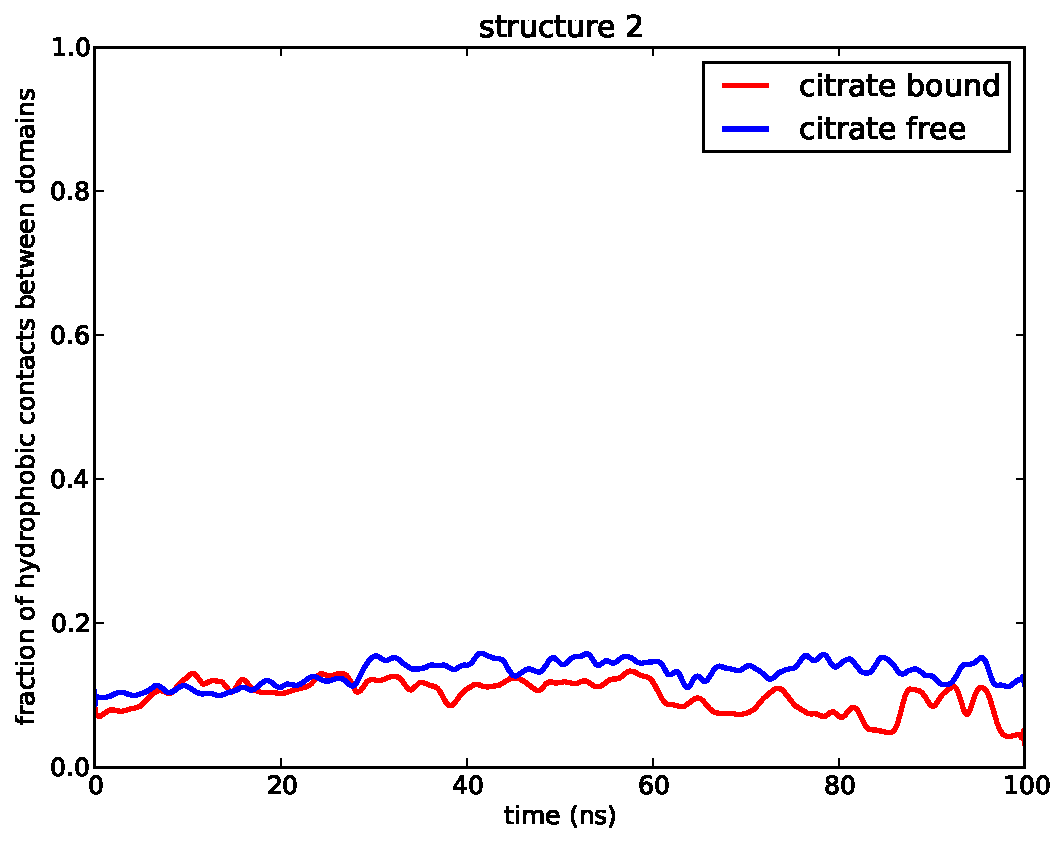
\includegraphics[width=\textwidth]{figures/Complex_hydrophobic_core/hydrophobic_cont_structure2.pdf}  
        d)
        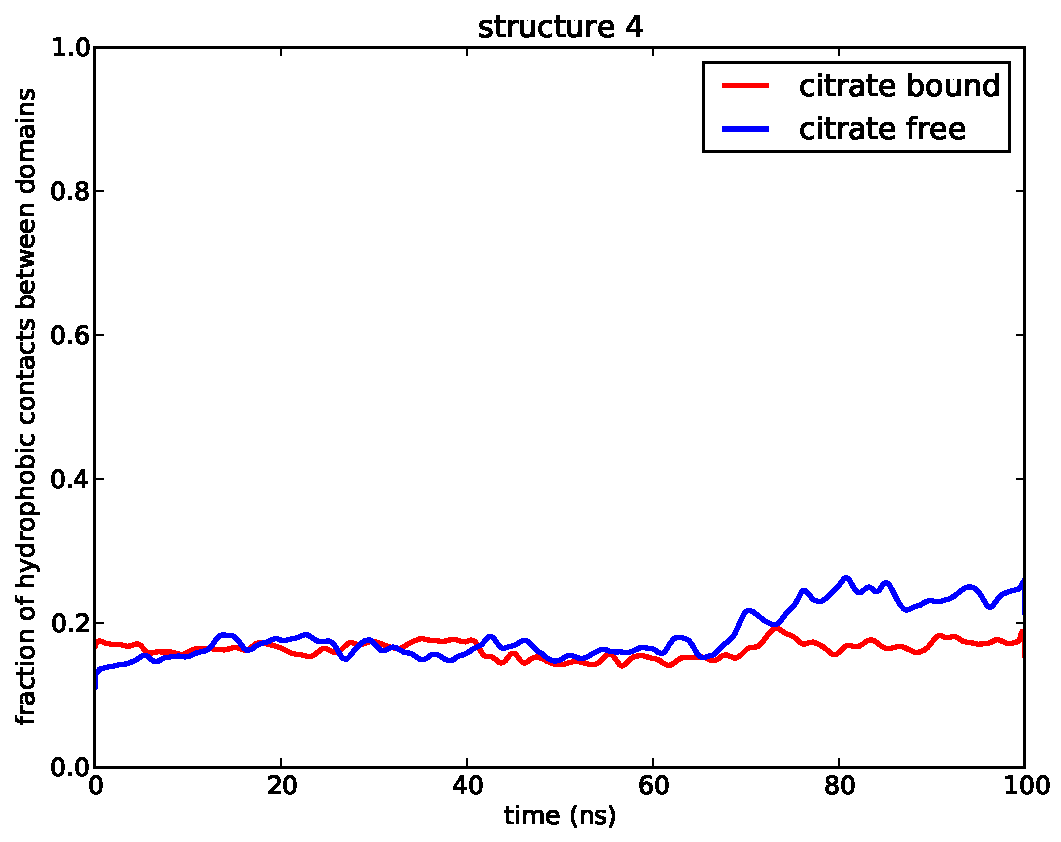
\includegraphics[width=\textwidth]{figures/Complex_hydrophobic_core/hydrophobic_cont_structure4.pdf}  
    \end{minipage}
    \caption{Fraction of hydrophobic contacts of the total number of contacts between the CitAP and BSLA domains.
        The data has been smoothed by a Gaussian window function to remove high frequent fluctuations for better visualizability.}
\label{fig:hydrophobic_contacts}
\end{figure}    




% hydrophobic cores
%\begin{figure}
%    \centering
%    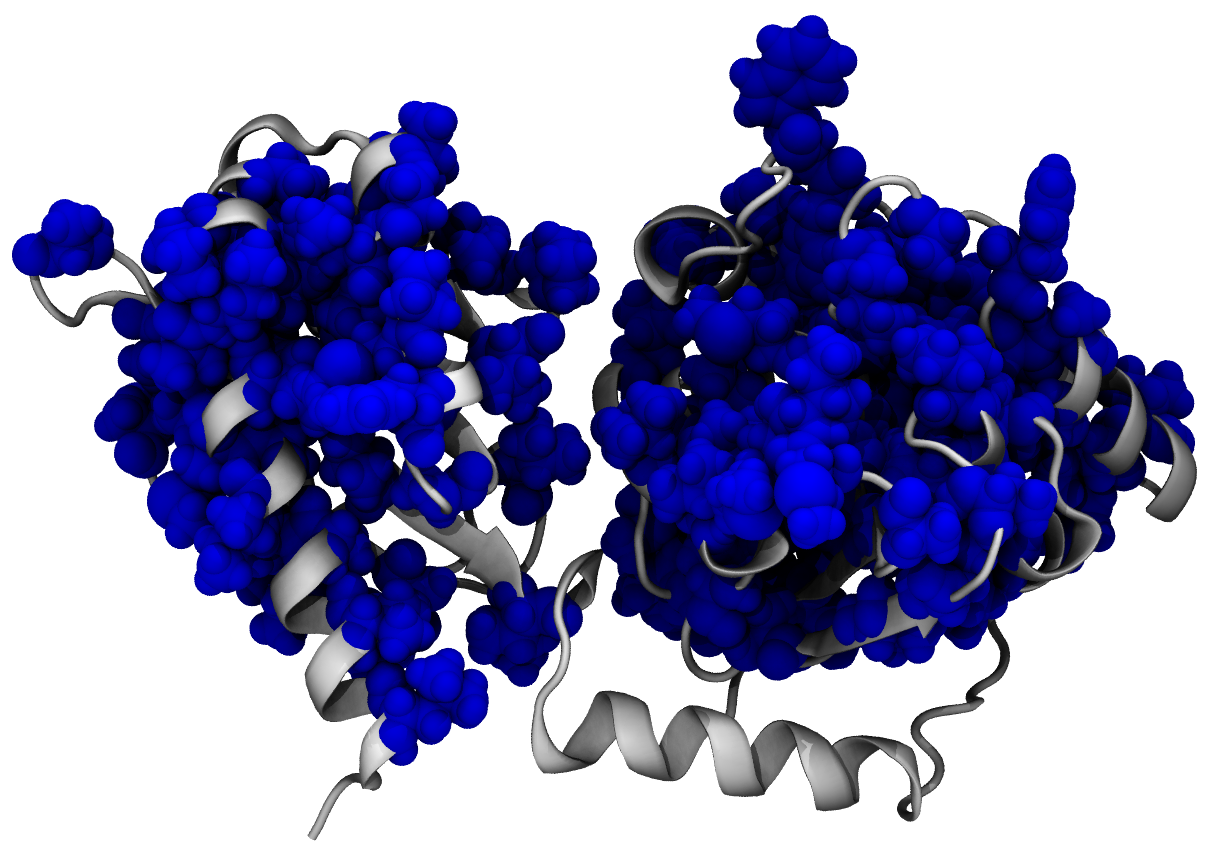
\includegraphics[width=0.7\textwidth]{figures/Complex_hydrophobic_core/hydrophobic_core.png}
%    \caption{Initial structure of fusion protein structure 3. The hydrophobic residues of the CitAP and the BSLA domains are shown in blue Van-der-Waals representations. Hydrophobic residues of the linker domain are not shown.}
%    \label{fig:hydrophobic_core}
%\end{figure} 

\begin{figure}
    \begin{minipage}[]{0.45\linewidth}
        \centering
        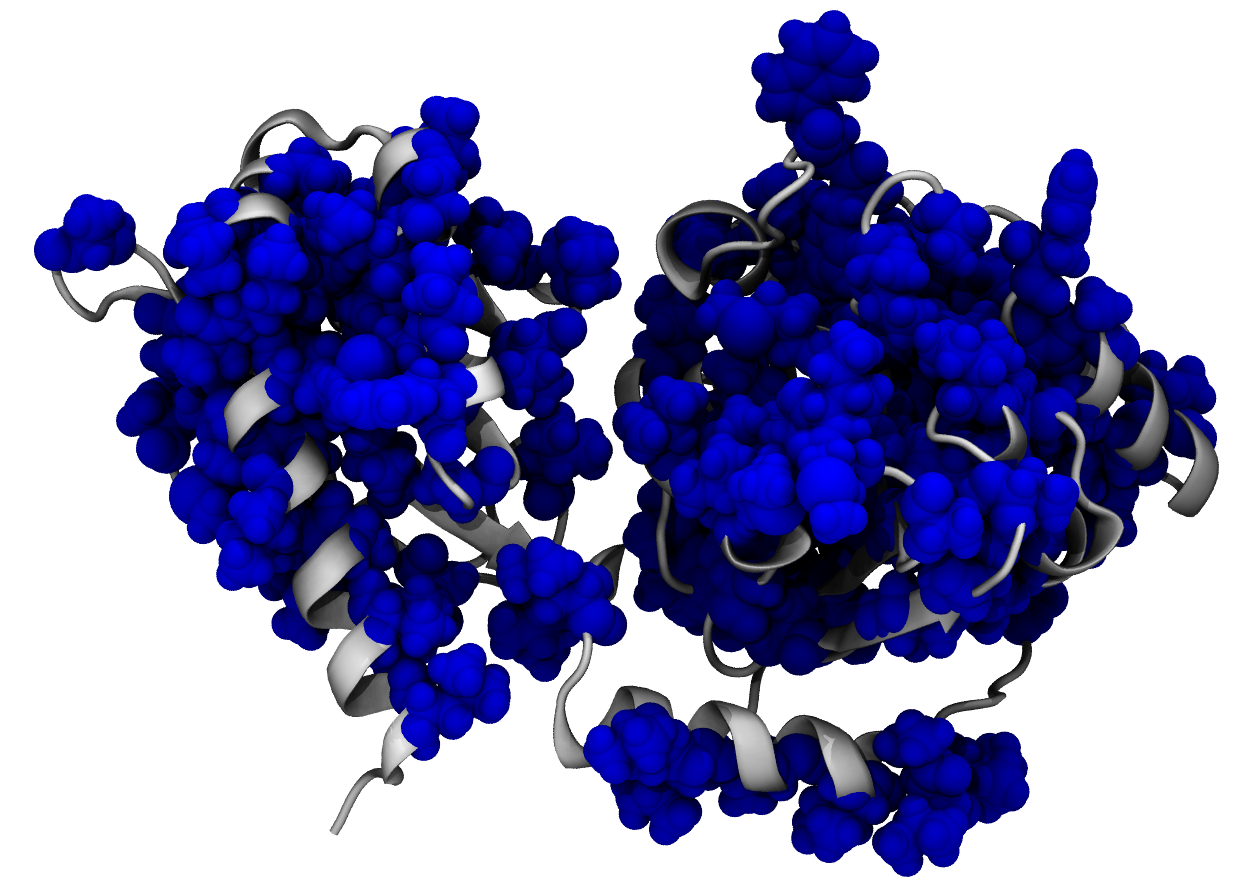
\includegraphics[width=\textwidth]{figures/Complex_hydrophobic_core/hydrophobic_core_linker.png}
    \end{minipage}
\hspace{0.5cm}
    \begin{minipage}[]{0.45\linewidth}
        \centering
        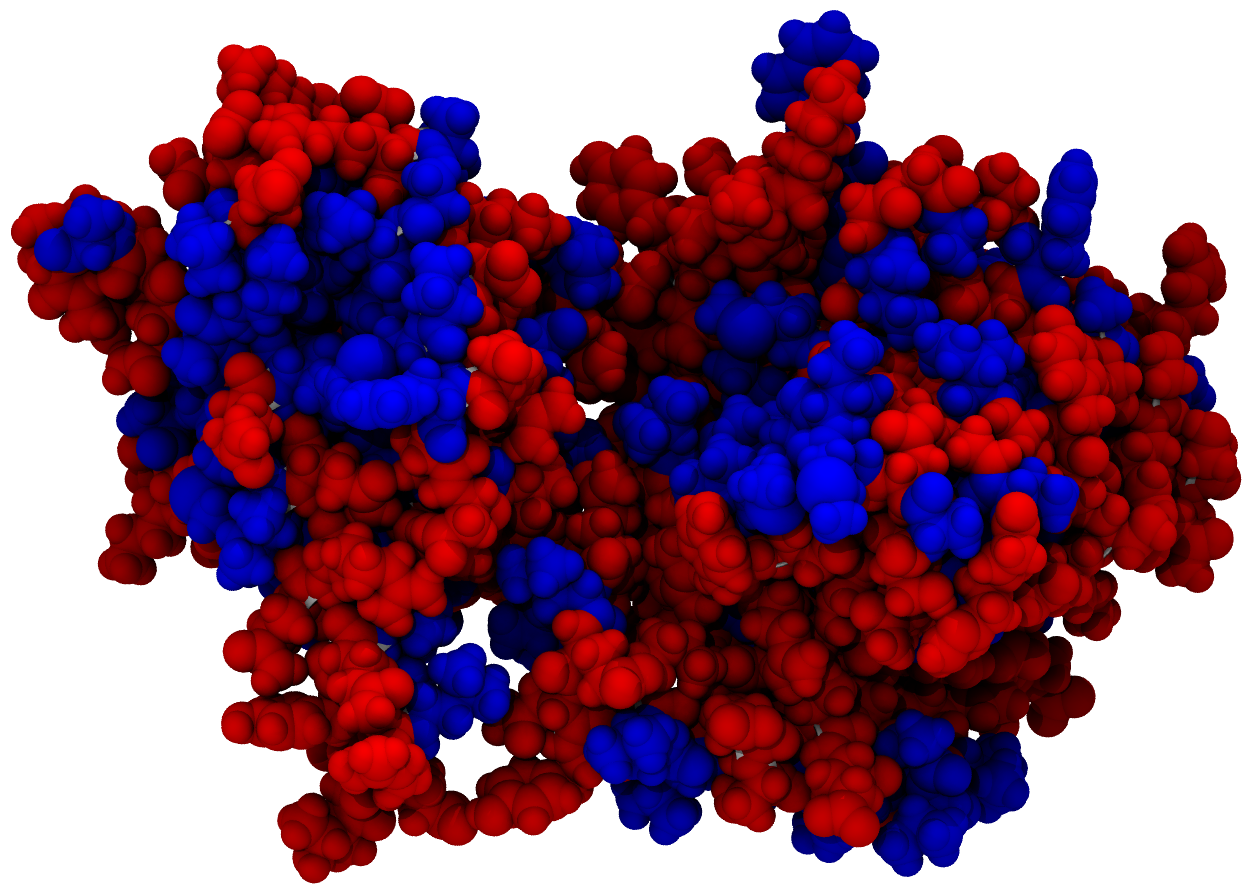
\includegraphics[width=\textwidth]{figures/Complex_hydrophobic_core/protein.png}
    \end{minipage}
    \caption{Initial structure of fusion protein structure 3. The left structure shows only hydrophobic residues in blue Van-der-Waals representation, the right structure shows in addition hydrophilic residues in red.}
    \label{fig:hydrophobic_core}
\end{figure}     



Figure \ref{fig:traj_reduced_coords} shows the MD trajectories of the four structures in their citrate bound and free forms in the reduced coordinate space described in section \ref{sec:DimRed}.
The two angles describing the relative CitAP and BSLA center of mass positions, $\phi_{Complex}$ and $\theta_{Complex}$, span a space in which the conformational evolution of the fusion protein is studied.
The deviation in the starting positions of the trajectories of corresponding citrate bound and free structures as indicated by the triangles are due to the equilibration procedure in which the backbone atom positions have been less and less restrained and therefore became more flexible.
In all four structures the CitAP and BSLA domains move relative to each other.
The trajectories of structure 2, 3 and 4, with and without citrate bound, are highly similar.
Structure 1 shows different trajectories, depending on whether citrate is bound or not.
This is in accordance with Figures \ref{fig:favourable_contacts} and \ref{fig:hydrophobic_contacts}, in which the citrate bound and citrate free trajectories are less similar than they are for the other three structures.
The two domains show considerably more flexibility for structures 1 and 3 than they do for structures 2 and 4.



% Trajectories in reduced coordinates
\begin{figure}
    \begin{minipage}[]{0.45\linewidth}
        \centering
        a)
        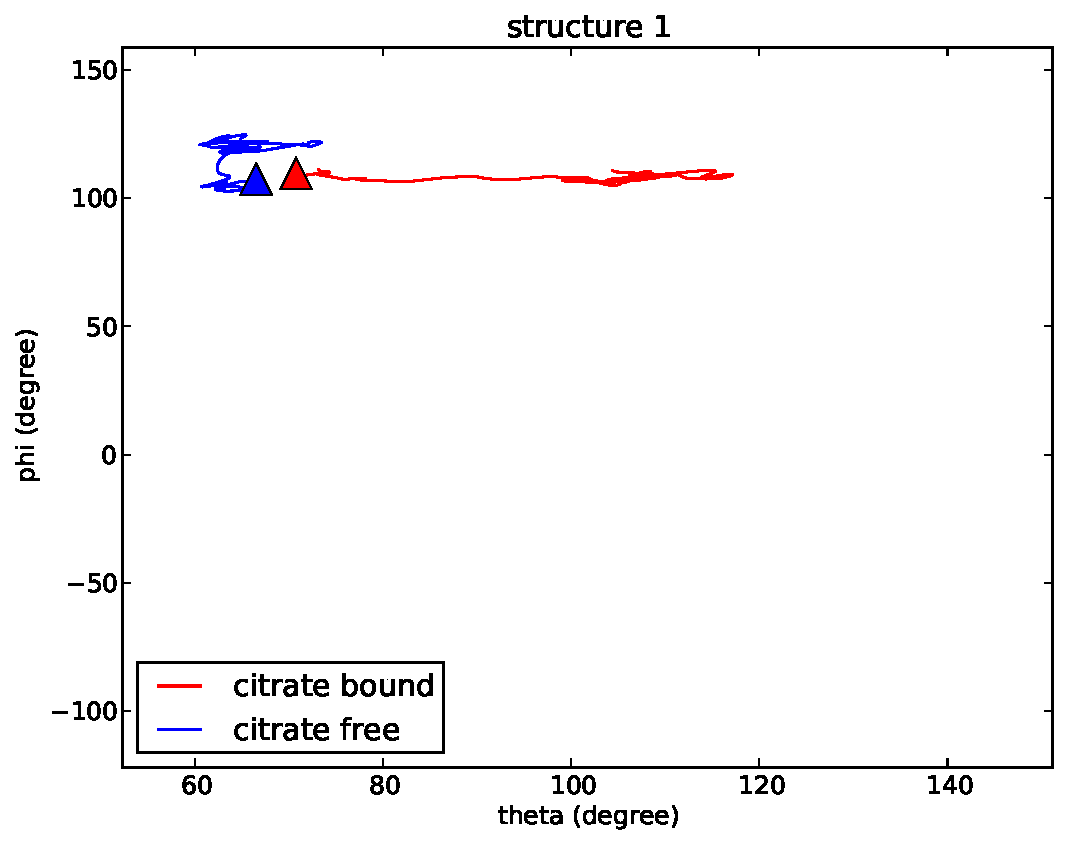
\includegraphics[width=\textwidth]{figures/Complex_trajectory/collecitve_coords_structure1.pdf}  
        c)
        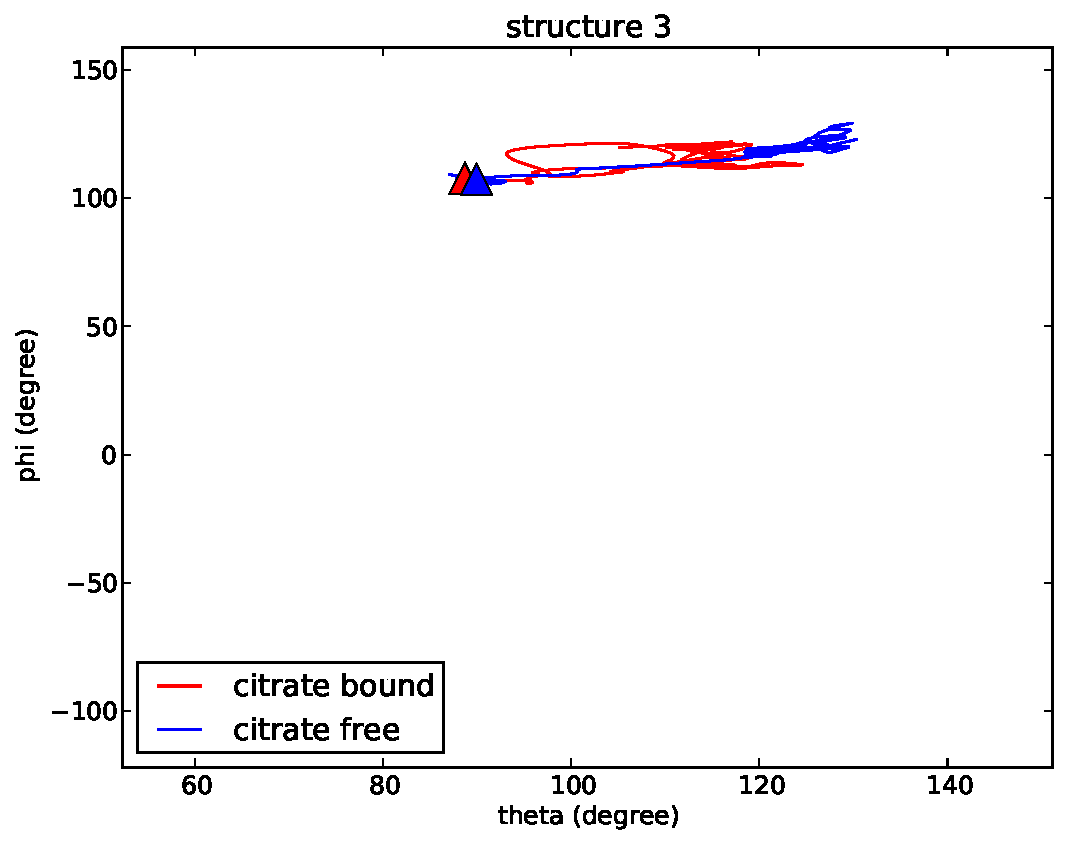
\includegraphics[width=\textwidth]{figures/Complex_trajectory/collecitve_coords_structure3.pdf}  
    \end{minipage}
\hspace{0.5cm}
    \begin{minipage}[]{0.45\linewidth}
        \centering
        b)
        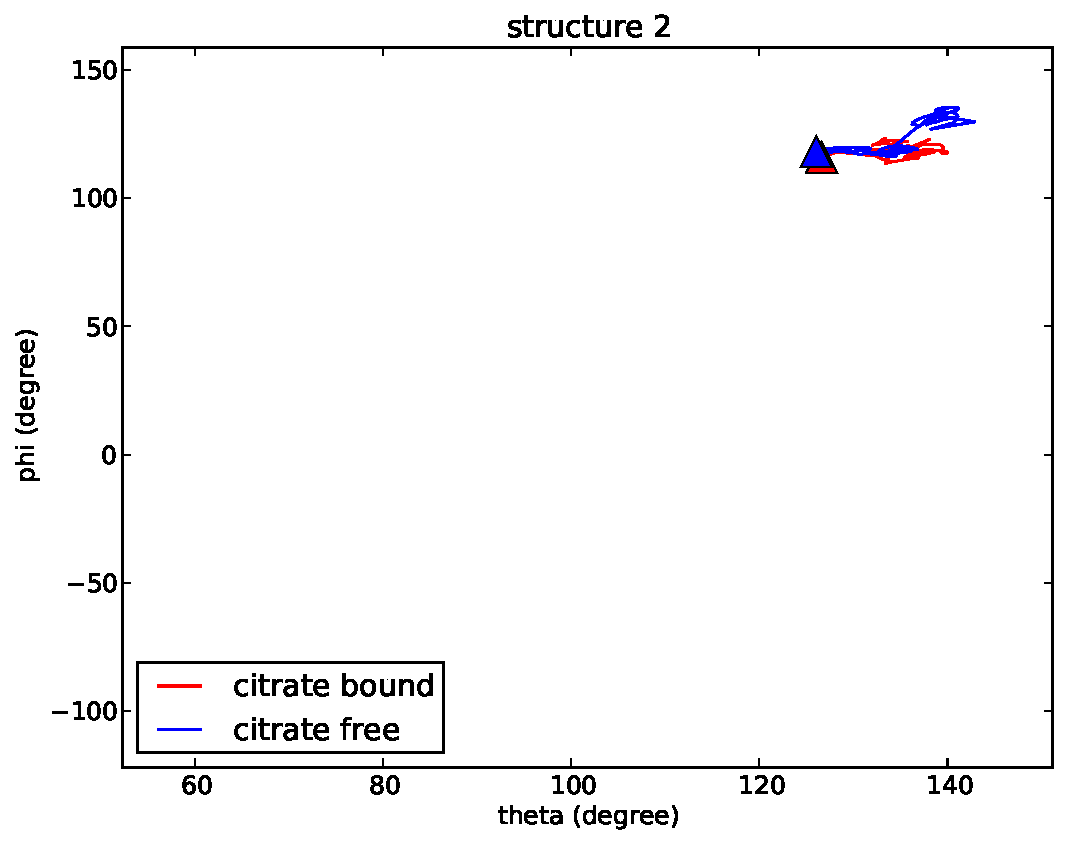
\includegraphics[width=\textwidth]{figures/Complex_trajectory/collecitve_coords_structure2.pdf}  
        d)
        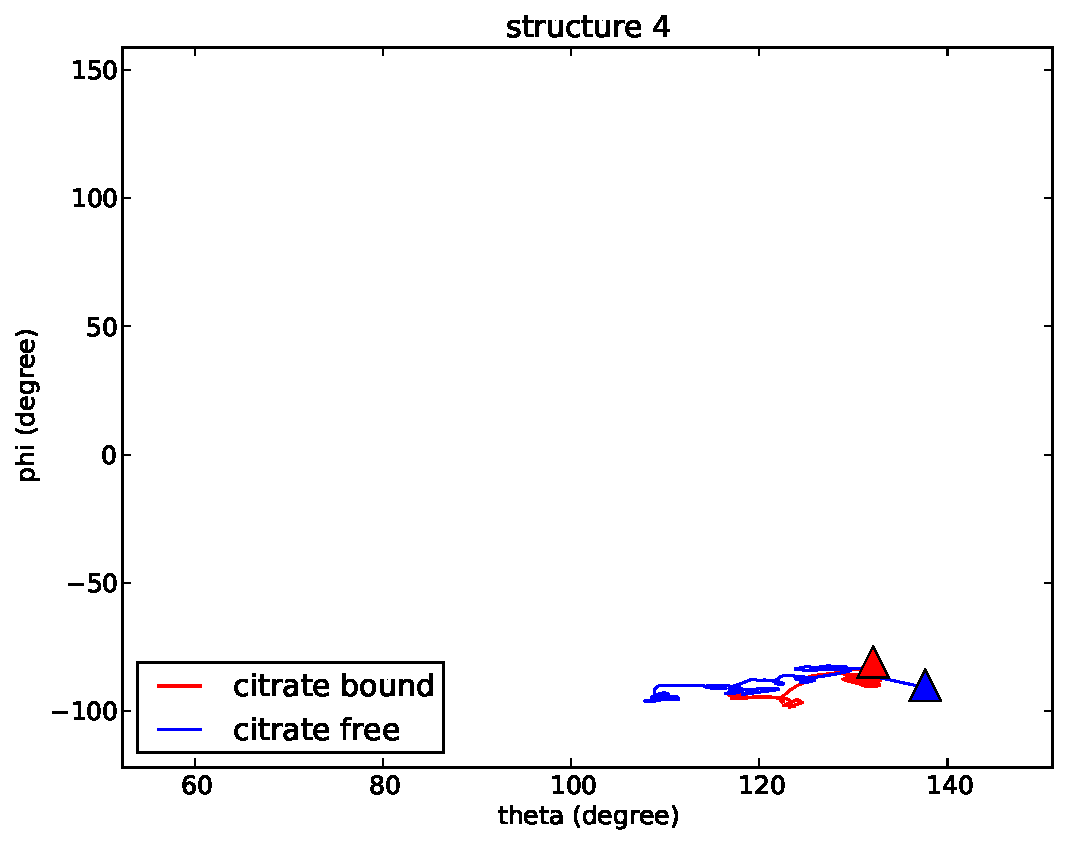
\includegraphics[width=\textwidth]{figures/Complex_trajectory/collecitve_coords_structure4.pdf}  
    \end{minipage}
    \caption{The MD trajectories are represented in a reduced coordinate space consisting only of the spherical angles $\phi_{Complex}$ and $\theta_{Complex}$ as defined in section \ref{sec:DimRed}.
        The starting points of the trajectories are indicated by triangles.}
\label{fig:traj_reduced_coords}
\end{figure}     


Only few experimental results exist that the simulations can be directly compared to. 
One experiment that has been performed in the group of Karl-Erich Jaeger is a measurement of the Tryptophan and Tyrosine fluorescence.
Tryptophan has been excited with radiation at 278 nm.
The emitted light intensity was measured for wavelengths between 290 and 380 nm.
The intensities at each wavelength are influenced by energy transfer from Tryptophan to Tyrosine residues.
Therefore the mutual orientations of and distances between Tryptophan and Tyrosine residues influence the emitted spectrum.
Figure \ref{fig:TyrTrp_fluorescence} shows that the fluorescence signal is altered by the presence or absence of citrate from the fusion protein, while it has no effect on the solo BSLA.
Neither does succinate as a reference probe show any influence on the fluorescence spectrum of solo BSLA nor of fusion protein.
This result indicates that citrate binding to the fusion protein triggers a conformational change that results in a change in Tryptophan to Tyrosine distances or orientations.
To compare the MD results to this experimental result, the minimum distance between any two Tryptophan and Tyrosine residues was analyzed.
This distance is shown in Figure \ref{fig:TyrTrp_distance} for all four fusion protein structures with and without citrate.
While structures 1 and 2 do not show a significant difference of the minimum Tyrosine to Tryptophan distance, structures 3 and 4 indicate such a conformational change.
Figure \ref{fig:TyrTrp_average} backs this result, as the variations of the average minimum Tyr/Trp distance for the citrate bound and citrate free simulations are insignificant for structures 1 and 2, while they are more pronounced for structures 3 and 4, although in opposite directions.
While the minimum Tyr/Trp distance increases during the simulation of structure 3 from the citrate free to the citrate bound case it decreases for structure 4.
The experimental fluorescence experiment shows that citrate binding to the fusion protein results in a drop of fluorescence intensity in the lower part of the measured spectrum.
This might be indicative for an increasing distance between Trosine and Tryptophan residues or an orientational change that makes energy transfer between those residue pairs less favourable.
Therefore structure 3 would be in accordance with experiment, as the average minimal Tyr/Trp distance increases from the citrate free to the citrate bound state.
Structure 4 on the other hand would then go against the experimental findings.
As the mutual Trp/Tyr orientations have not been taken into account, there is also a possibility left for structures 1 and 2 to be in accordance with the experimentally measured fluorescence change.

 

% Tyr/Trp fluorescence experiment
\begin{figure}
    \centering
    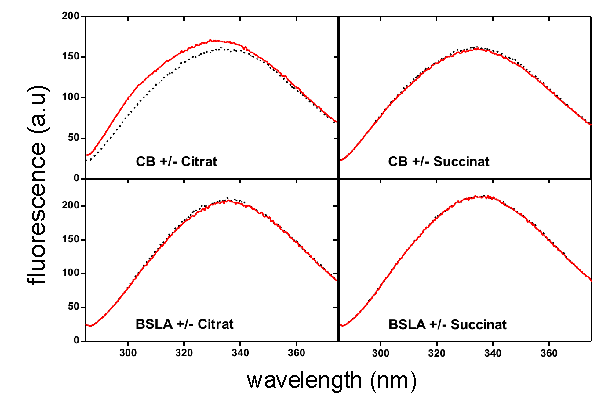
\includegraphics[width=0.8\textwidth]{figures/TyrTrp/TyrTrp_experiment.pdf}
    \caption{Change of Tryptophan and Tyrosine fluorescence changes due to citrate and succinate in solo BSLA and fused CitAP--BSLA (CB).
        Excitation happened at 278 nm.
        The addition of citrate to the fusion protein resulted in a drop of fluorescence in the lower part of the measured spectrum.}
    \label{fig:TyrTrp_fluorescence}
\end{figure}        



% Tyr/Trp minimum distances
\begin{figure}
    \begin{minipage}[]{0.45\linewidth}
        \centering
        a)
        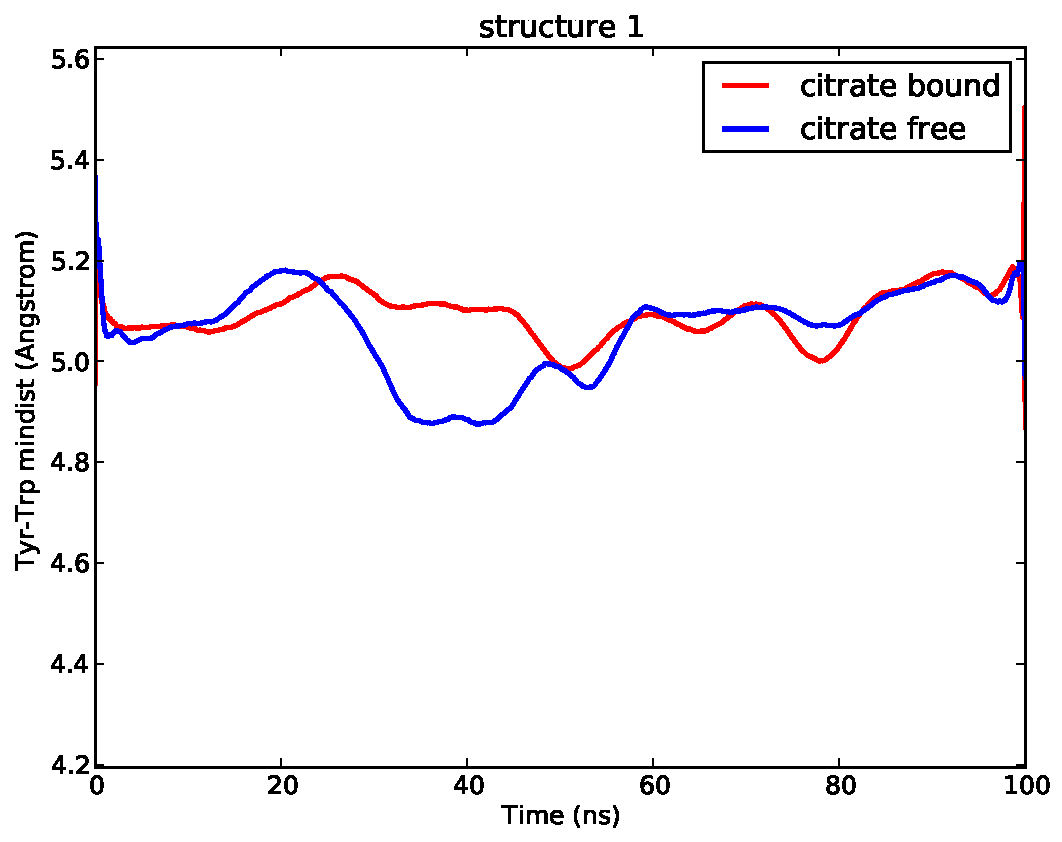
\includegraphics[width=\textwidth]{figures/TyrTrp/mindist_TyrTrp_structure0.pdf}  
        c)
        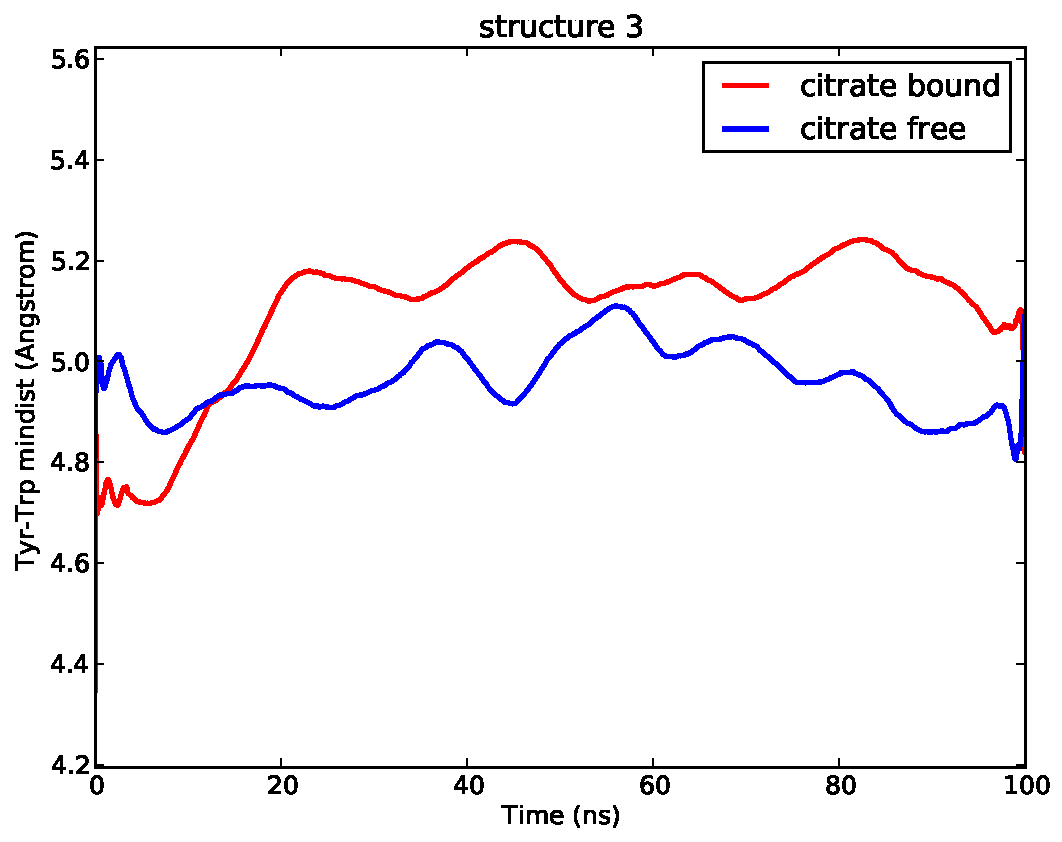
\includegraphics[width=\textwidth]{figures/TyrTrp/mindist_TyrTrp_structure2.pdf}  
    \end{minipage}
\hspace{0.5cm}
    \begin{minipage}[]{0.45\linewidth}
        \centering
        b)
        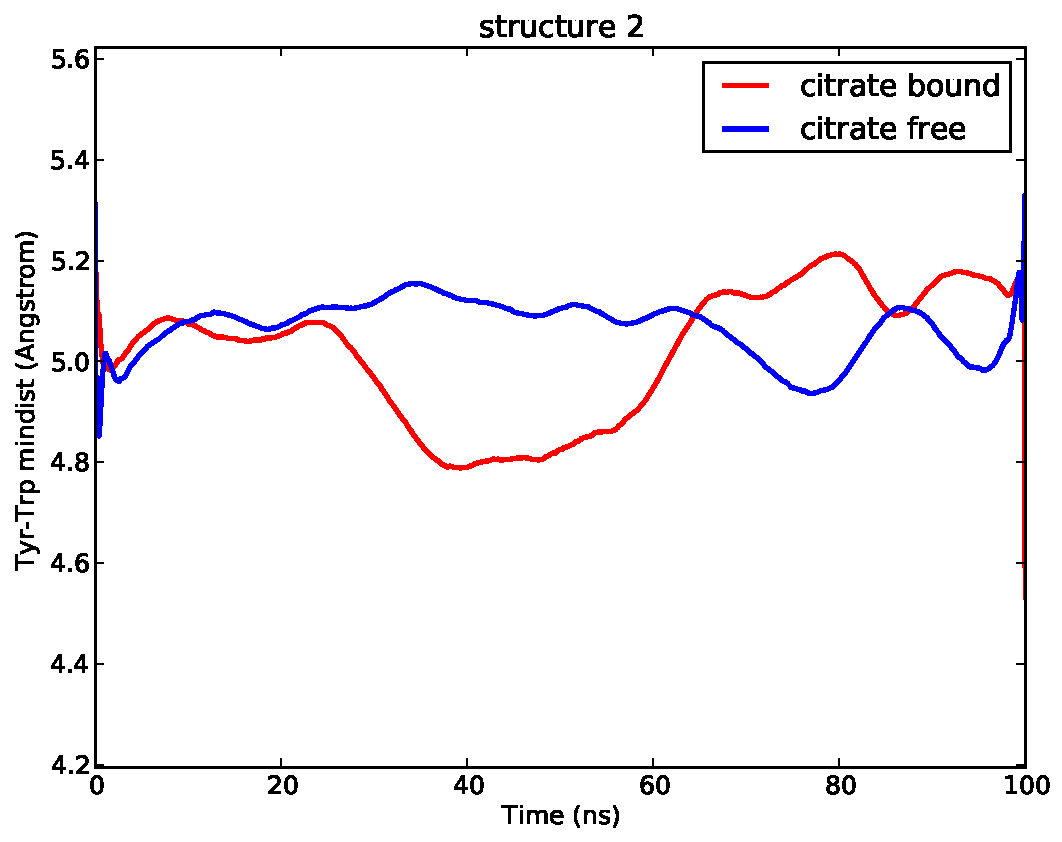
\includegraphics[width=\textwidth]{figures/TyrTrp/mindist_TyrTrp_structure1.pdf} 
        d)
        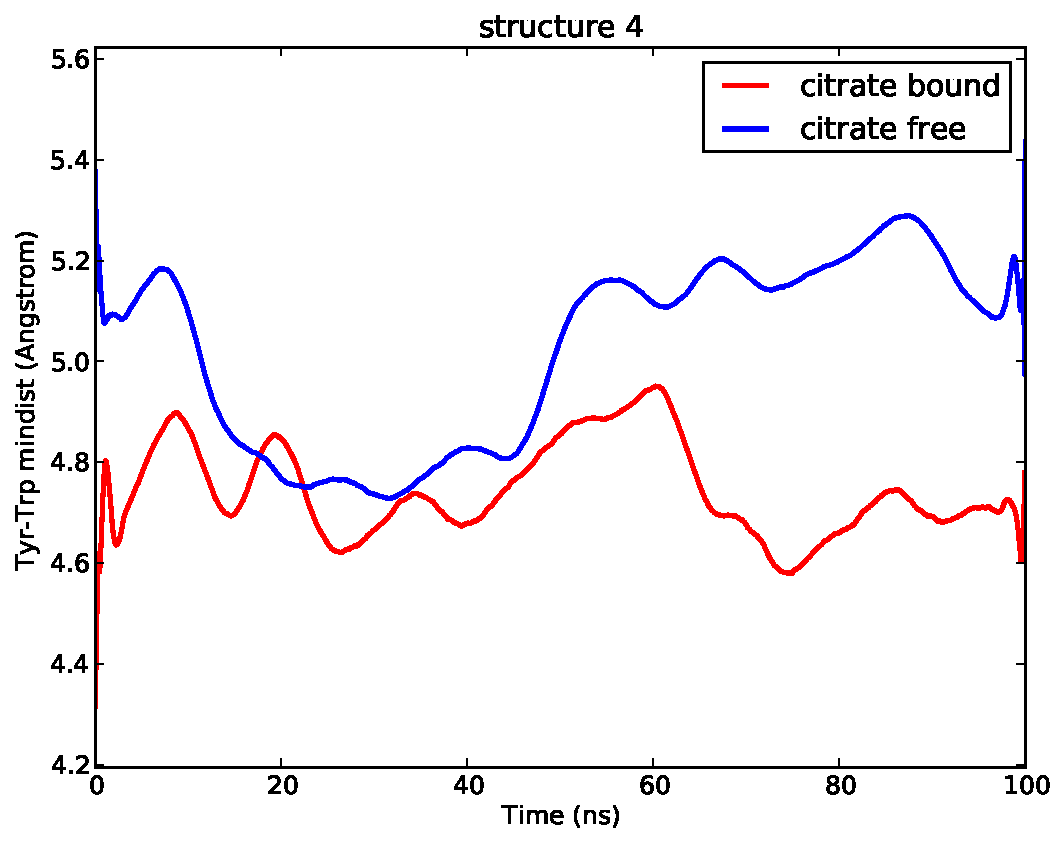
\includegraphics[width=\textwidth]{figures/TyrTrp/mindist_TyrTrp_structure3.pdf}  
    \end{minipage}
    \caption{Minimum distance between Tyrosine and Tryptophan residues during the MD trajectories of each structure.
        A difference between citrate bound and citrate free structures would be in accordance with the experimental results of the Jaeger group (Figure \ref{fig:TyrTrp_fluorescence}).
        The data has been smoothed by a gaussian window function to remove high frequent fluctuations for better visualizability.}
\label{fig:TyrTrp_distance}
\end{figure}  



% Tyr/Trp average minimal distance
\begin{figure}
    \centering
    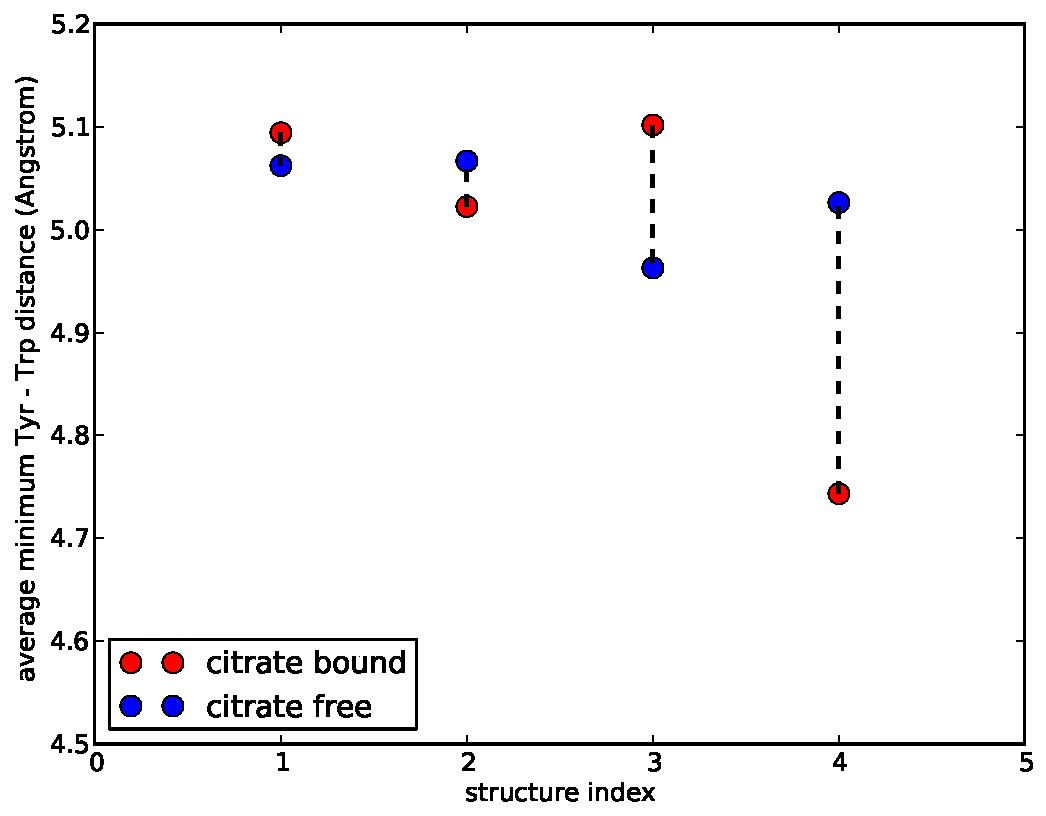
\includegraphics[width=0.6\textwidth]{figures/TyrTrp/average_mindist_TyrTrp.pdf}
    \caption{Averages of the minimal distances between Tyrosine and Tryptophan as displayed in Figure \ref{fig:TyrTrp_distance}.}
    \label{fig:TyrTrp_average}
\end{figure}         



          


Further experimental data exists about the effect of citrate binding on the activity of BSLA, as displayed in Figure \ref{fig:BSLAactivity}.
One possible explanation for this effect might be a change in the BSLA binding pocket conformation triggered by citrate binding.
Visual inspection of the MD trajectories showed that the distance between the side chains of ASP133 and HIS156 is the strongest varying distance in the BSLA binding pocket (residue numbering according to solo BSLA).
As hydrogen bonding between these two residues stabilizes the tetrahedral intermediate structure of the substrate, an increase in this distance might be related to a disruption of BSLA activity.
As it is already known from the study of the solo CitAP binding pocket, that its geometry depends on the presence or absence of citrate, the distance between LEU102:N to GLU56:C$_{\alpha}$ of the CitAP binding pocket has been related to the afore mentioned distance of the BSLA binding pocket.
Figure \ref{fig:active_site_mean_sd} shows the mean of the last 50 ns of each simulation and the standard deviation of these distances for each structure in their citrate bound and citrate free forms.
The BSLA binding pocket distance is a measure for the disruption of its active site and therefore a large distance is thought to correspond to a low BSLA activity.
The standard deviations of the distances are a measure for the pocket flexibility, which is assumed to be correlated to the BSLA activity.
The standard deviation of the corresponding distance in the solo BSLA MD run is very small (0.07 \r{A}ngstrom).
Structure 1 and 3 exhibit a positive correlation for the two active site distances.
When their CitAP pockets open up in the absence of citrate and become more flexible, the BSLA pocket also gains flexibility and the ASP133--HIS156 distance increases.
In structure 2 the CitAP binding pocket opens up even in the presence of citrate and this is even more true for structure 4.
Interestingly, while the CitAP binding pocket is similarly open on average in the citrate bound and free simulations, the BSLA pocket is on average much wider in the citrate bound case.
The standard deviation of these two cases is moderate.
Both binding pocket distances of structure 4 have a large standard deviation in both, the citrate free and bound form.
Citrate binding seems even to destabilize the CitAP pocket further, while it has a stabilizing effect on the BSLA active site.





% CitAP BSLA active site distance
\begin{figure}
    \begin{minipage}[]{0.45\linewidth}
        \centering
        a)
        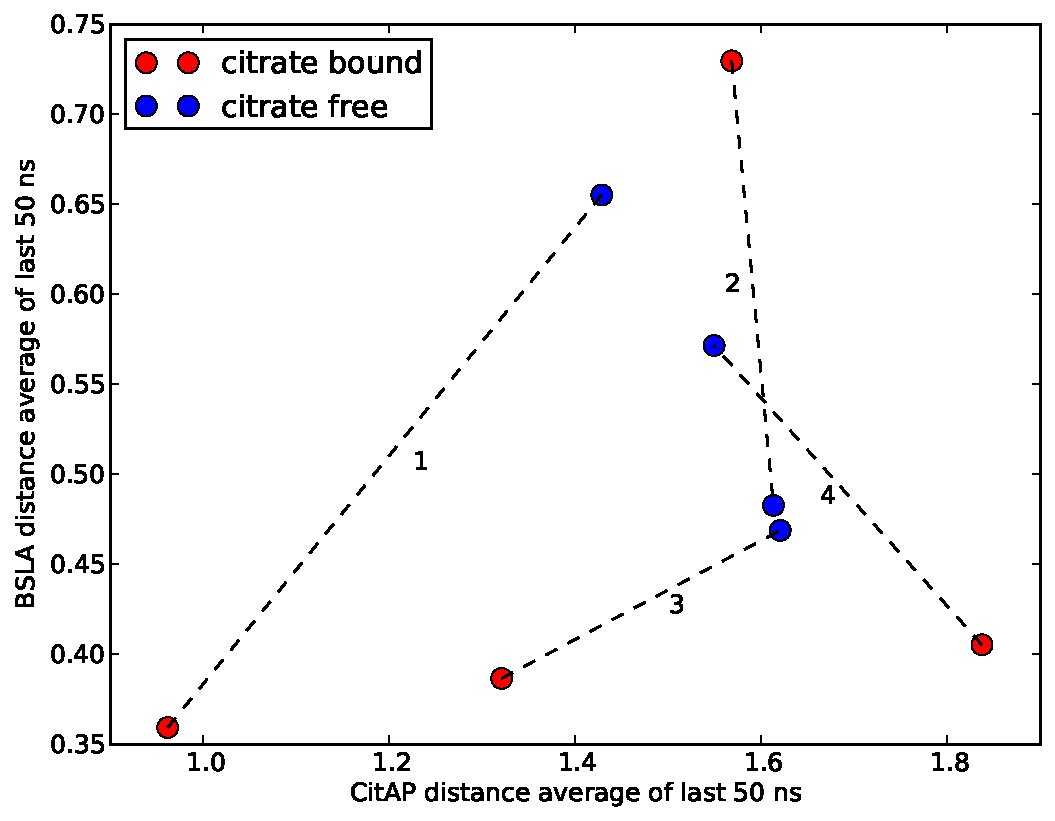
\includegraphics[width=\textwidth]{figures/CitAP_BSLA_distance/BSLA_CitAP_analyzed_with_average_of_last_50_ns.pdf}  
    \end{minipage}
\hspace{0.5cm}
    \begin{minipage}[]{0.45\linewidth}
        \centering
        b)
        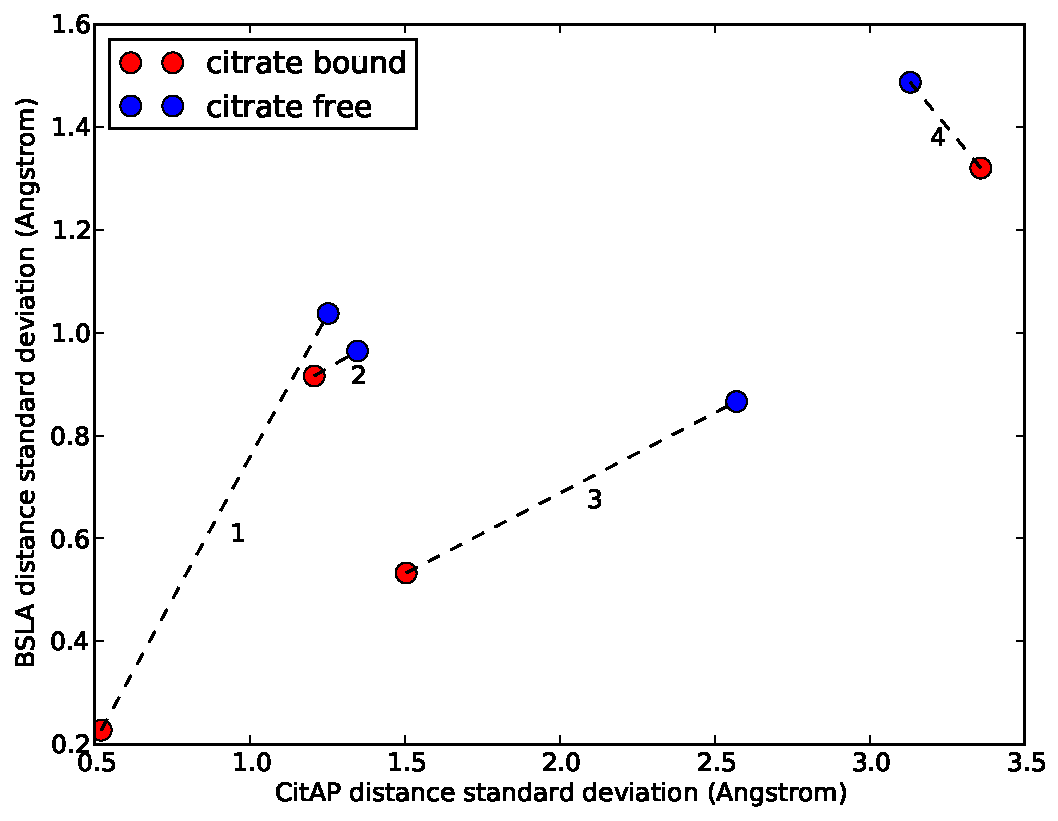
\includegraphics[width=\textwidth]{figures/CitAP_BSLA_distance/BSLA_CitAP_analyzed_with_standard_deviation.pdf}  
    \end{minipage}
    \caption{\textbf{a)} Averages of the last 50 ns of each MD simulation of the active site ASP133 to HIS156 distance in the BSLA domain versus the active site LEU102:N to GLU56:C$_{\alpha}$ distance of the CitAP domain (residue numbering with respect to the solo structures).
        The numbers indicate the corresponding structure.
        \textbf{b)} Standard deviation of the distance from a).}
\label{fig:active_site_mean_sd}
\end{figure}     



Figure \ref{fig:active_site_bound_distribution} shows contour plots of the distributions of CitAP and BSLA active site distances for the citrate bound simulations.
The BSLA pockets stay closed for all citrate bound simulations, although structure 2 seems to have a second stable state in a slightly more opened conformation.
The CitAP pocket stays tightly closed as expected for the citrate bound MD runs for structures 2 and 3, while it is slightly more flexible for structure 1.
Structure 4 is even in the citrate bound case a lot more open than the other structures.
 



% CitAP BSLA bound active site distance distributions
\begin{figure}
    \begin{minipage}[]{0.45\linewidth}
        \centering
        a)
        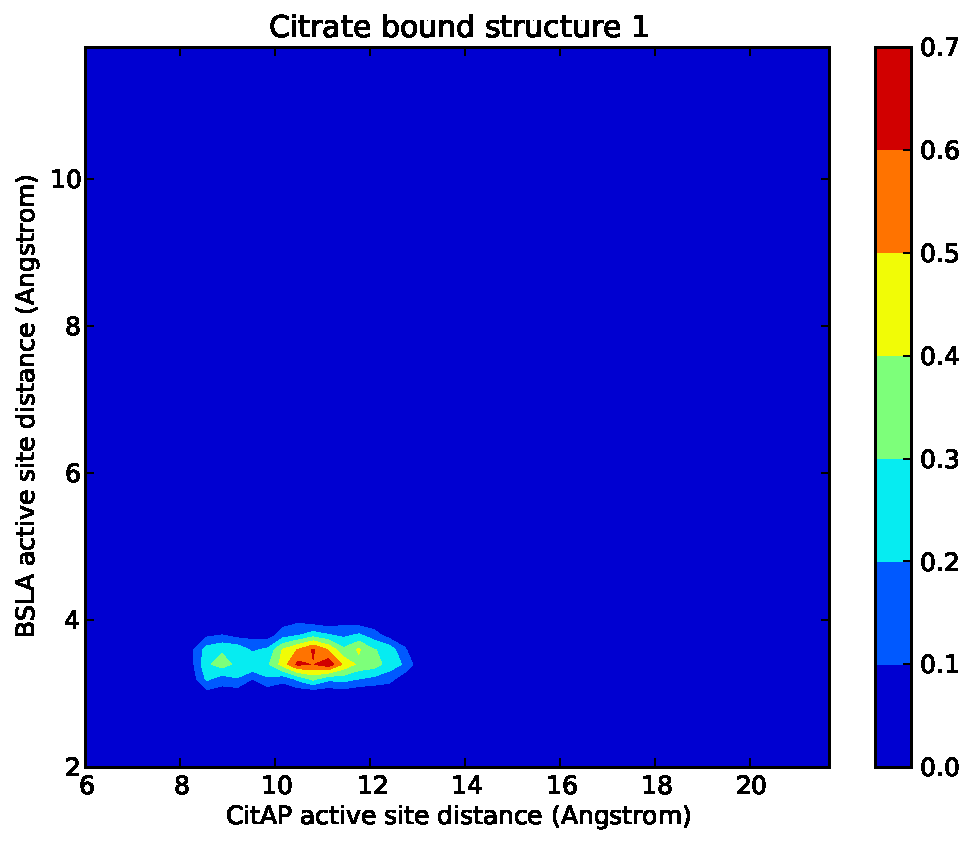
\includegraphics[width=\textwidth]{figures/CitAP_BSLA_distance/BSLA_CitAP_distance_bound_contour_structure1.pdf}  
        %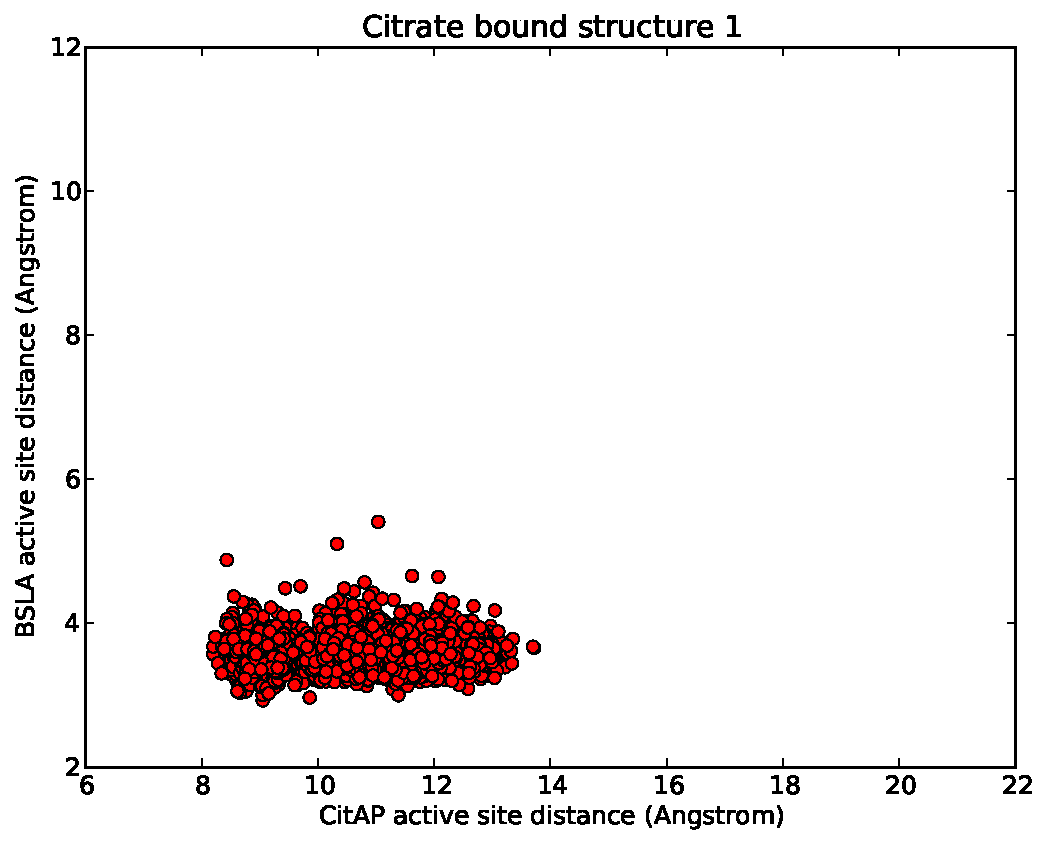
\includegraphics[width=\textwidth]{figures/CitAP_BSLA_distance/BSLA_CitAP_distance_bound_structure1.pdf}  
        c)
        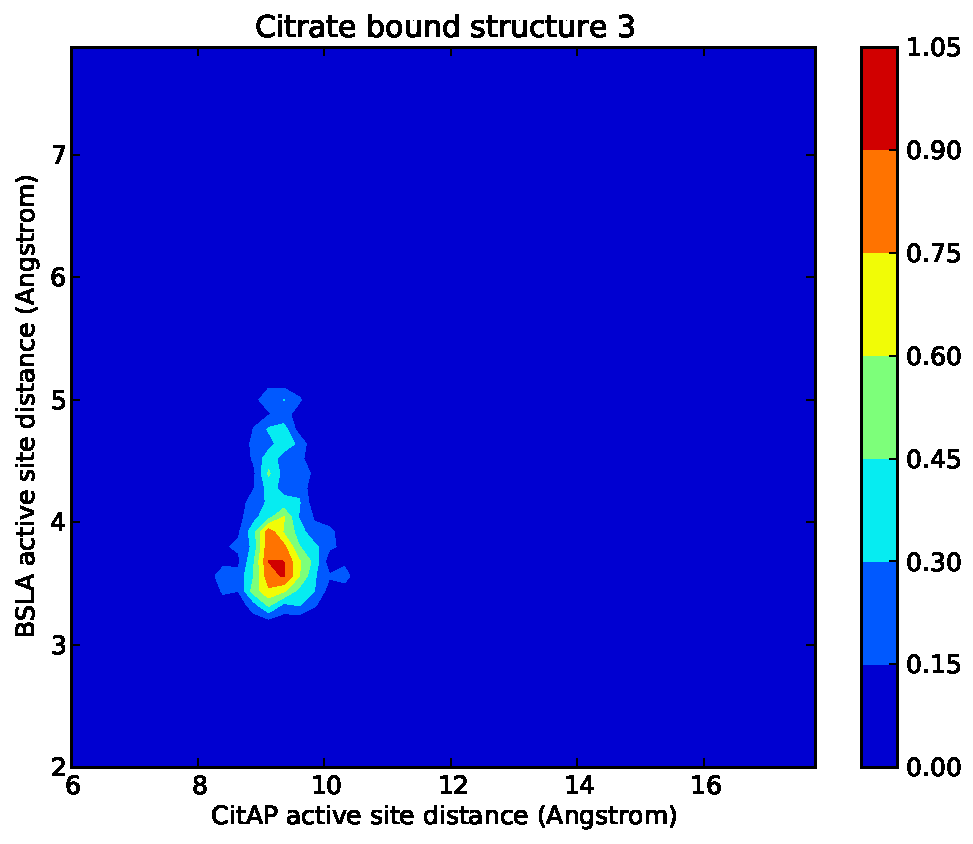
\includegraphics[width=\textwidth]{figures/CitAP_BSLA_distance/BSLA_CitAP_distance_bound_contour_structure3.pdf}  
        %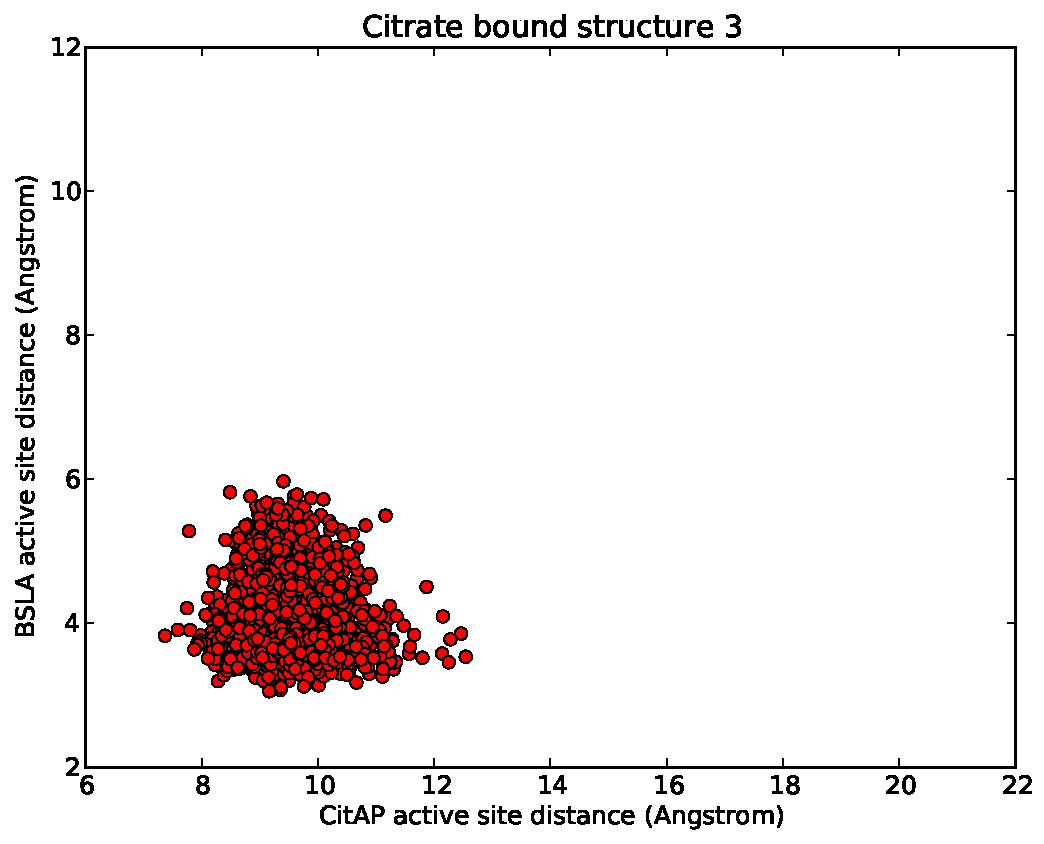
\includegraphics[width=\textwidth]{figures/CitAP_BSLA_distance/BSLA_CitAP_distance_bound_structure3.pdf}  
    \end{minipage}
\hspace{0.5cm}
    \begin{minipage}[]{0.45\linewidth}
        \centering
        b)
        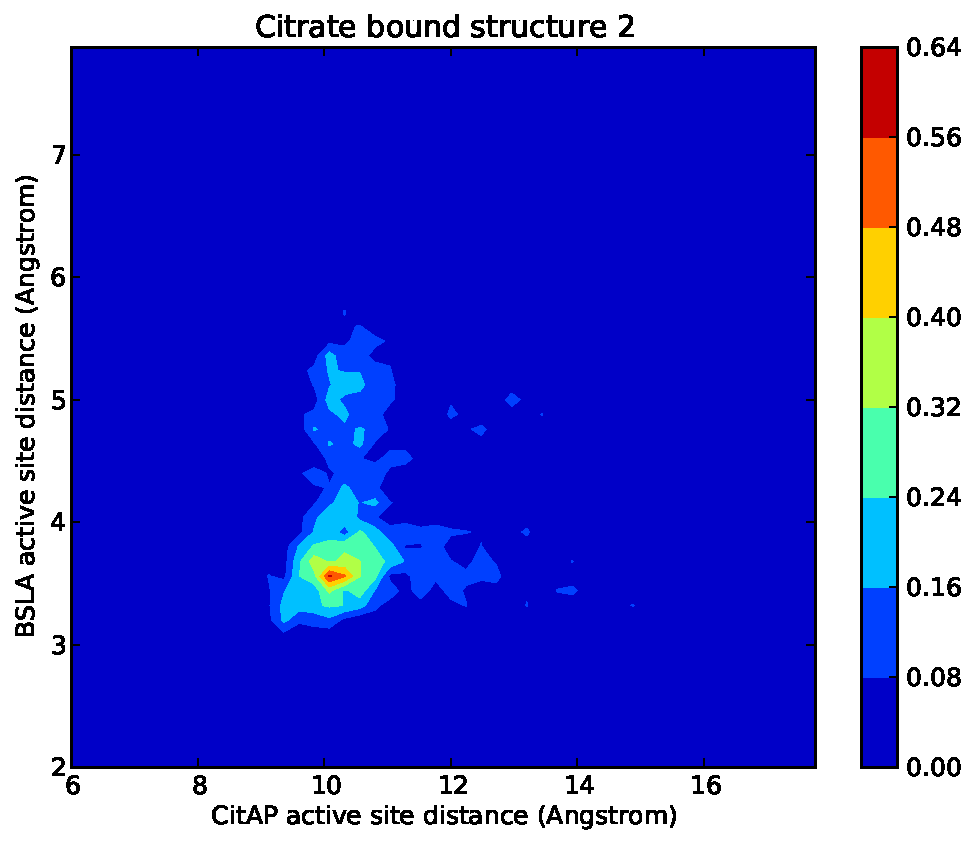
\includegraphics[width=\textwidth]{figures/CitAP_BSLA_distance/BSLA_CitAP_distance_bound_contour_structure2.pdf}  
        %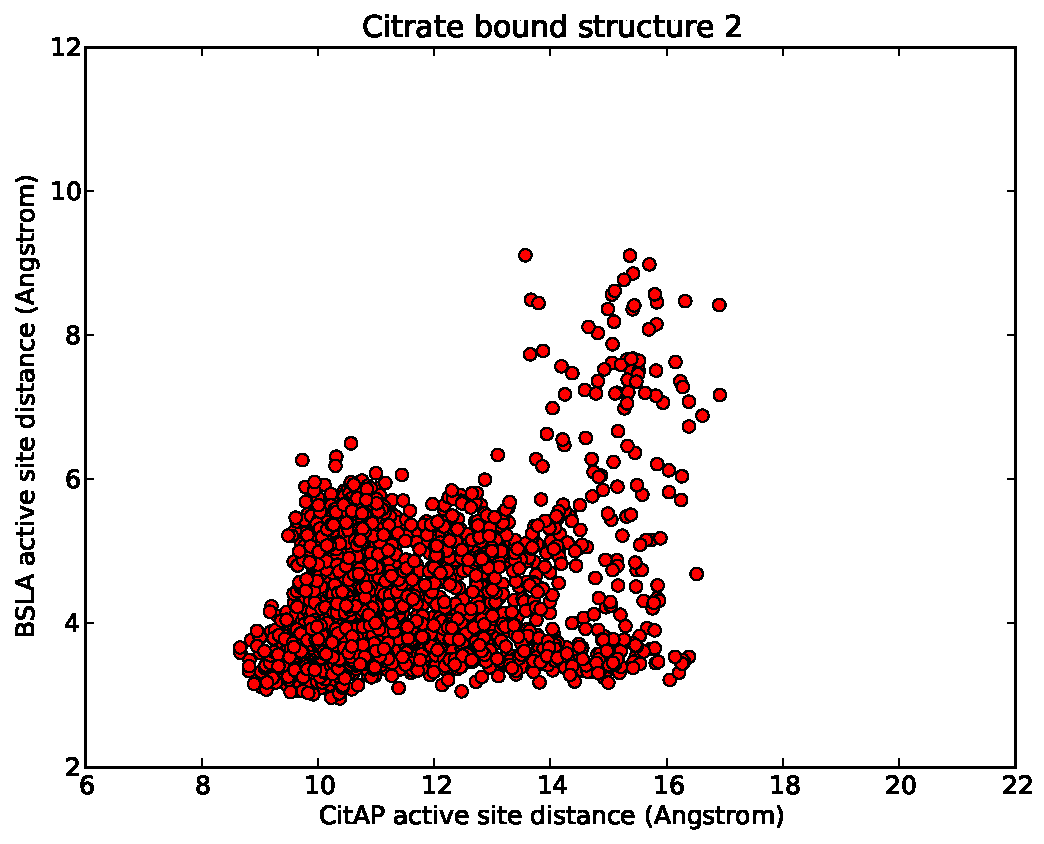
\includegraphics[width=\textwidth]{figures/CitAP_BSLA_distance/BSLA_CitAP_distance_bound_structure2.pdf}  
        d)
        \includegraphics[width=\textwidth]{figures/CitAP_BSLA_distance/BSLA_CitAP_distance_bound_contour_structure4.pdf}  
        %\includegraphics[width=\textwidth]{figures/CitAP_BSLA_distance/BSLA_CitAP_distance_bound_structure4.pdf}  
    \end{minipage}
    \caption{Distribution of active site distances for citrate bound structures (ASP133 to HIS156 in BSLA, LEU102:N to GLU56:C$_{\alpha}$ in CitAP, numbering with respect to the solo structures).
    The distributions are normalized to integrate to unity.}
\label{fig:active_site_bound_distribution}
\end{figure}      



Figure \ref{fig:active_site_free_distribution} displays analogous distributions for the citrate free simulations.
Structure 1 and 2 have remarkably stable CitAP binding pockets in the absence of citrate.
One possible origin is the fact that the minor loop, which opens up in the solo CitAP simulations, has some interactions with the BSLA domain.
But as this is also true for structure 3, which even has a very stable open conformation in the absence of citrate, this is unlikely to be the only source of this effect.
Structure 4 has for both binding pocket distances the largest flexibility among all structures.
    




% CitAP BSLA free active site distance distributions
\begin{figure}
    \begin{minipage}[]{0.45\linewidth}
        \centering
        a)
        \includegraphics[width=\textwidth]{figures/CitAP_BSLA_distance/BSLA_CitAP_distance_free_contour_structure1.pdf}  
        %\includegraphics[width=\textwidth]{figures/CitAP_BSLA_distance/BSLA_CitAP_distance_free_structure1.pdf}  
        c)
        \includegraphics[width=\textwidth]{figures/CitAP_BSLA_distance/BSLA_CitAP_distance_free_contour_structure3.pdf}  
        %\includegraphics[width=\textwidth]{figures/CitAP_BSLA_distance/BSLA_CitAP_distance_free_structure3.pdf}  
    \end{minipage}
\hspace{0.5cm}
    \begin{minipage}[]{0.45\linewidth}
        \centering
        b)
        \includegraphics[width=\textwidth]{figures/CitAP_BSLA_distance/BSLA_CitAP_distance_free_contour_structure2.pdf}  
        %\includegraphics[width=\textwidth]{figures/CitAP_BSLA_distance/BSLA_CitAP_distance_free_structure2.pdf}  
        d)
        \includegraphics[width=\textwidth]{figures/CitAP_BSLA_distance/BSLA_CitAP_distance_free_contour_structure4.pdf}  
        %\includegraphics[width=\textwidth]{figures/CitAP_BSLA_distance/BSLA_CitAP_distance_free_structure4.pdf}  
    \end{minipage}
    \caption{Distribution of active site distances for citrate free structures (ASP133 to HIS156 in BSLA, LEU102:N to GLU56:C$_{\alpha}$ in CitAP, numbering with respect to the solo structures).
    The distributions are normalized to integrate to unity.}
\label{fig:active_site_free_distribution}
\end{figure}       





% ============================================================================ %

\section{Discussion \& Conclusion}

The MD simulations of the solo CitAP and BSLA domains are very promising.
BSLA not only stays folded and close to its crystal structure conformation through the whole course of the simulation, it is moreover very stable with a small RMSF for the core structure and only slightly larger fluctuations in loop regions in contact with the solvent.
This is indicative for simulations at or near equilibrium.
The active site, especially the conformation of the catalytic triad residues is very stable, with only small fluctuations in the mutual distances and orientations.
This is an indication that the proposed reaction mechanism for ester hydrolysis, that is based on the crystal structure, is likely to be correct.

The solo CitAP simulations are far more interesting.
The hypothesized open conformation in the absence of citrate could be confirmed in so far, as the minor loop covering the binding pocket opens up during the 100 ns MD trajectory, while it stays tightly closed in the citrate bound state.
Unfortunately the long timescale of binding kinetics does not permit a simulation to start at the open conformation withe goal to observe a closing of the pocket in the presence of citrate.
It is however hard to detect the proposed piston mechanism that is induced by the opening of the minor loop.
The neighbouring $\beta$-sheet is hypothesized to bend upon active site opening.
This motion is small in magnitude, so that no theory can yet be based on this conformational change.

From the Basin Hopping results, four possible structures have been selected.
Due to lack of experimental data it is unknown which structural properties the fusion protein possesses in reality.
The secondary structures of all four of these structures are stable for at least 100 ns.
Interestingly, the two protein domains make only a moderate fraction of favourable contacts, although both possess hydrophobic patches on their solvent interface.
One reason might simply be a geometric misfit of the hydrophobic interface domains, that would make major conformational rearrangements necessary.
These cannot be observed during the simulation timescales.
It would be interesting to try to dock the two isolated domains by protein--protein docking to each other and compare the result to the GMIN output structures to see if these sample the most favourable inter-protein interactions.

In general the two domains maintain their separated hydrophobic cores.
This is due to the restrictions imposed on the Basin Hopping algorithm, as only the linker domain was allowed to adapt new conformations.
It is however questionable whether the real structure of the fusion protein might not undergo more drastic rearrangements to fuse the two hydrophobic cores.
In that respect it would be very interesting to see whether this structure would still possess undisrupted active sites.

The MD trajectories in reduced coordinate space show that the two protein domains significantly move relative to each other for three of the four structures (1, 3 and 4).
This is likely an indication of an unequilibrated system.
The equilibration time necessary for the rearrangements to complete and the fusion protein to reach its native state, might simply be too long to be accessible by MD simulations and range in regime of protein folding simulations.


Assuming that the structures under study contain the native fusion protein conformation, or at least one of several possible, as these might as well be an ensemble of multiple conformations, it is instructive to compare structural properties to experimental data.
While structure 3 is in accordance with the experimental fluorescence measurements, structure 4 clearly goes against them.
Structures 1 and 2 do not show any Tyr/Trp distance change.
But as structure 3 also undergoes one of the largest conformational rearrangements between the two protein domains as outlined earlier,
The Tyr/Trp distance change might simply be a result of domain movements not present in the equilibrated structure.

The comparison of the introduced active site distances give interesting insights.
The BSLA distance is very stable for the solo BSLA and the solo CitAP distance follows the proposed dynamics.
But in the fusion protein, the CitAP distance is not as stable in the citrate bound case for three of the four structures.
One possible explanation for this observation are the additional interactions that the CitAP domain has in the fusion protein, especially as the minor loop makes direct contact with the BSLA domain in structures 1, 2 and 3.
But interestingly enough the CitAP distance is largest and most variable for structure 4, in which the CitAP binding pocket points away from the BSLA domain and is solvent exposed, similar to the solo structure.
In the citrate free simulations, the CitAP active site is not opening up in structures 1 and 2, again possibly due to interactions with BSLA.
Citrate free structure 3 has two well separated stable states.
This feature has not been observed for any other structure and seems to be a unique feature of the citrate free state of structure 3.
Finally, the BSLA pocket is fairly stable in all citrate free simulations of structures 1, 2 and 3, but exhibits much more flexibility in the citrate free simulation of structure 4.

All four structures therefore show different binding pocket dynamics.
It was not possible to relate these dynamics directly to the theory of the CitAP influence on BSLA activity.
The assumption is that the CitAP pocket is closed and inflexible when citrate is bound and much more flexible and open in the absence of citrate.
The closed conformation might trigger a conformational change in the BSLA domain, presumably by the piston mechanism described for the CitAP domain.
This conformational change might then in turn disrupt the BSLA active site, or at least introduce more flexibility, which in turn reduces the BSLA activity.
This effect could not be observed for any of the structures.
Structures 1 and 3 even show the exact opposite behaviour, where the more flexible citrate free structure correlates with a more (and not less) flexible BSLA pocket.

As experimental evidence on the true conformation of the fusion protein is still lacking, the validity of the reported results of the fusion protein dynamics remains rather uncertain.


% ============================================================================ %

\section{Outlook}

The lack of experimental data complicates the investigation of the fusion protein structure and dynamics.
A full crystal structure of the complex, or detailed NMR data would be the most desirable structural information, which would directly enable solid computational investigations into the mechanism of citrate triggered down-regulation of BSLA activity.
Many other experimental methods could however result in measured quantities that could directly be compared to computer simulations.
Small angle X-ray or neutron scattering could for example give some insights into the true shape of the fusion protein.
Fluorescence resonance energy transfer (FRET) could be used to generate data on inter-protein distances, which could then be compared directly to the generated structures and result in an refinement of the set of starting structures for molecular simulations.


% ============================================================================ %

\pagebreak

\section{Acknowledgments} 

\section{Declaration of Authorship}

% ============================================================================ %


% ============================================================================ %


% ============================================================================ %



% ============================================================================ %

\pagebreak

\singlespacing
\small

\bibliographystyle{unsrt}
\bibliography{masterthesis}
 
% ============================================================================ %

\end{document}
 
